\documentclass[kpfonts]{patmorin}
\listfiles
\usepackage{pat}
\usepackage{paralist}
\usepackage{dsfont}  % for \mathds{A}
\usepackage[utf8x]{inputenc}
\usepackage{skull}

\usepackage{graphicx}
\usepackage[noend]{algorithmic}

\usepackage[normalem]{ulem}
\usepackage{cancel}
\usepackage{enumitem}

\usepackage[longnamesfirst,numbers,sort&compress]{natbib}

% Taken from
% https://tex.stackexchange.com/questions/42726/align-but-show-one-equation-number-at-the-end
\newcommand\numberthis{\addtocounter{equation}{1}\tag{\theequation}}


\setlength{\parskip}{1ex}

\title{\MakeUppercase{(Layered) Partitions versus Decompositions}}
\author{}

\DeclareMathOperator{\tw}{tw}
\DeclareMathOperator{\stw}{stw}
\DeclareMathOperator{\ltw}{ltw}
\DeclareMathOperator{\pw}{pw}
\DeclareMathOperator{\lpw}{lpw}
\DeclareMathOperator{\lhptw}{lhp-tw}
\DeclareMathOperator{\lhppw}{lhp-pw}


\title{\MakeUppercase{Asymptotically Optimal Vertex 2-Ranking of Planar Graphs}}
\author{Prosenjit Bose, Vida Dujmović, Mehrnoosh Javarsineh, and Pat Morin}

\newcommand{\trn}{\chi_2}
\newcommand{\dtcn}{\bar{\chi}_2}
\newcommand{\htrn}{\hat{\chi}_2}
\newcommand{\scn}{\chi_{\star}}

\newtheorem{othertheorem}{Theorem}
\renewcommand*{\theothertheorem}{\Alph{othertheorem}}
\crefname{othertheorem}{Theorem}{Theorem}

\newtheoremstyle{named}{}{}{\itshape}{}{\bfseries}{.}{.5em}{#3}
\theoremstyle{named}
\newtheorem*{namedtheorem}{Unused}

\newcommand{\weirdref}[2]{\cref{#1}#2}
\newcommand{\weirdlabel}[2]{\label{#1-#1}}

\pagenumbering{roman}
\begin{document}
\begin{titlepage}
\maketitle

\begin{abstract}
  A (vertex) 2-ranking is a labelling $\varphi:V(G)\to\N$ of the vertices of a graph $G$ with integer colours so that for any path $v_0,\ldots,v_r$ of length $r\le 2$, $\max\{\varphi(v_0),\ldots,\varphi(v_r)\}$ appears exactly once in the sequence $\varphi(v_0),\ldots,\varphi(v_r)$.  We show that every $n$-vertex planar graph has a 2-ranking using $O(\log n/\log\log\log n)$ colours and this is tight; for some $n$-vertex planar graphs, any 2-ranking requires $\Omega(\log n/\log\log\log n)$ colours.  This result also extends to bounded genus graphs.

  In developing this proof we obtain optimal bounds on the number of colours needed for 2-ranking $t$-trees and simple $t$-trees (this includes planar 3-trees and outerplanar graphs).  These upper bounds are constructive and give $O(n\log n)$-time algorithms.  Additional results that come from our techniques include new sublogarithmic upper bounds on the number of colours needed for 2-rankings of bounded genus graphs, apex minor-free graphs, and $k$-planar graphs.
\end{abstract}
\end{titlepage}

\tableofcontents

\newpage
\pagenumbering{arabic}

\section{Introduction}

A sequence of integers $\phi_0,\ldots,\phi_r$ is \emph{ranked} if $\max\{\phi_0,\ldots,\phi_r\}$ occurs exactly once in $\phi_0,\ldots,\phi_r$. A \emph{colouring} $\varphi:V(G)\to \N$ of a graph $G$ is an \emph{$\ell$-ranking} if, for every path $v_0,\ldots,v_r$ in $G$ of length\footnote{The length of a path $v_0,\ldots,v_r$ is the number, $r$, of edges in the path.} at most $\ell$ the sequence $\varphi(v_0),\ldots,\varphi(v_r)$ is ranked.\footnote{An alternative, but equivalent, condition is that for every path $v_0,\ldots,v_r$ of length $r\le\ell$,
\begin{inparaenum}[(i)]
   \item $\varphi(v_0)\neq \varphi(v_r)$; or
   \item $\max\{\varphi(v_0),\ldots,\varphi(v_r)\} > \varphi(v_0)$.
\end{inparaenum}
}
The $\ell$-ranking number $\chi_\ell(G)$ is the minimum integer $k$ such that $G$ has a $\ell$-ranking $\varphi:V(G)\to \{1,\ldots,k\}$.

Two cases have received special attention: An $\infty$-ranking is called a \emph{vertex ranking} or \emph{ordered colouring}. The parameter $\chi_\infty(G)$ is called the \emph{vertex ranking number} of $G$ and has applications to matrix factorization \cite{bodlaender.gilbert.ea:approximating,duff.reid:multifrontal,liu:role,dereniowski.kubale:cholesky}, VLSI layout \cite{leiserson:area,sen.deng.ea:on}, and the analysis of online algorithms \cite{even.smorodinsky:hitting}. The case $\ell=2$ has also received special attention \cite{almeter.demircan.ea:graph,karpas.neiman.ea:on,shalu.antony:complexity}. A $2$-ranking is called a \emph{unique-superior colouring} (abbreviated \emph{us-colouring}) by \citet{karpas.neiman.ea:on} who prove the following result:

\setcounter{othertheorem}{19}
\begin{othertheorem}[\cite{karpas.neiman.ea:on}]\label{trees}
    For every $n$-vertex tree $T$, $\trn(T)\in O(\log n/\log\log n)$ and this is asymptotically optimal: for infinitely many values of $n$, there exists an $n$-vertex tree $T$ with $\trn(T)\in\Omega(\log n/\log\log n)$.
\end{othertheorem}

The same authors prove the following result for planar graphs:

\setcounter{othertheorem}{15}
\begin{othertheorem}[\cite{karpas.neiman.ea:on}]\label{planar-graphs}
    For every $n$-vertex planar graph $G$, $\trn(G)\in O(\log n)$.
\end{othertheorem}

Since every tree is a planar graph and no better lower bound is known for planar graphs, this leaves an obvious question:  Which is the correct bound for planar graphs, $\log n$ or $\log n/\log\log n$?  As it turns out, neither is correct.  Let $\log x :=\log_2 x$ denote the binary logarithm of $x$ and define $\log^{(0)}x:=x$ and, for any integer $i>0$, let $\log^{(i)}x:=\log(\log^{(i-1)} x)$. We prove:


\begin{thm}\label{planar}
    For every $n$-vertex planar graph $G$, $\trn(G)\in O(\log n/\log^{(3)} n)$ and this is asymptotically optimal: for infinitely many values of $n$, there exists an $n$-vertex planar graph $G$ with $\trn(G)\in \Omega(\log n/\log^{(3)} n)$
\end{thm}

Our proof of the upper bound in \cref{planar} makes use of a recent \emph{product structure theorem} of \citet{dujmovic.joret.ea:planar} which states that every planar graph $G$ is a subgraph of $H\boxtimes K_3\boxtimes P$ where $H$ is a planar $3$-tree, $K_3$ is a 3-cycle, $P$ is a path, and $\boxtimes$ denotes the strong graph product.\footnote{Definitions of $t$-trees, simple $t$-trees, treewidth, simple treewidth, and strong graph product appear later, in \cref{sec:basics}.}  To apply this theorem, we prove the following result:

\begin{thm}\label{simple-t-trees}
    For every $n$-vertex simple $t$-tree $H$, $\trn(H) \in O(\log n/\log^{(t)}n)$.
    and this is asymptotically optimal: for all integer $t\ge 1$ and infinitely many values of $n$, there exists an $n$-vertex simple $t$-tree $H$ with $\trn(H)\in\Omega(\log n/\log^{(t)} n)$.
\end{thm}

\Cref{simple-t-trees} is immediately relevant because a 3-tree is planar if and only if it is a simple $3$-tree. Therefore, the lower bound in \cref{simple-t-trees} immediately implies the lower bound in \cref{planar} since it shows the existence of $n$-vertex planar graphs with $\trn(T)\in\Omega(\log n/\log^{(t)} n)$.

To obtain the upper bound in \cref{planar}, we apply \cref{simple-t-trees} to the graph $H$ defined by the product structure theorem along with a simple lemma which shows that, for any two graphs $G_1$ and $G_2$, $\trn(G_1\boxtimes G_2)\le \trn(G_1)\cdot\dtcn(G_2)$ where $\dtcn(G_2)$ is the \emph{distance-2 colouring number} of $G_2$;  the minimum number of colours needed to colour $G_2$ so that the endpoints of each non-trivial path of length at most 2 have different colours.  It is easy to see that $\dtcn(K_3\times P)\le 9$, so $\trn(H\boxtimes K_3\boxtimes P)\le 9\trn(H)$.

%
% For general $t$-trees, we obtain the following generalization of \cref{trees}:
%
% \begin{thm}\label{t-trees}
%     For every fixed $t$ and every $n$-vertex $t$-tree, $\trn(G) \in O(\log n/\log^{(t+1)}(n)$ and this is asymptotically optimal: for infinitely many values of $n$, there exists an $n$-vertex $t$-tree $T$ with $\trn(T)\in\Omega(\log n/\log^{(t+1)} n)$.
% \end{thm}

% Observe that, for $t=2$, the lower bound in \cref{t-trees} matches the upper bounds in \cref{planar,three-trees}.  Since every $2$-tree is planar and is, in fact, a subgraph of a planar $3$-tree, the lower bound in \cref{t-trees} establishes the lower bounds in \cref{planar,three-trees}.

Every (not-necessarily simple) $t$-tree is the subgraph of some simple $(t+1)$-tree. Therefore, the upper bound in \cref{simple-t-trees} implies the (upper bound in) the following generalization of \cref{trees}:

\begin{thm}\label{t-trees}
    For every fixed $t$ and every $n$-vertex $t$-tree $H$, $\trn(H) \in O(\log n/\log^{(t+1)}(n)$ and this is asymptotically optimal: for infinitely many values of $n$, there exists an $n$-vertex $t$-tree $H$ with $\trn(H)\in\Omega(\log n/\log^{(t+1)} n)$.
\end{thm}

The lower bound in \cref{t-trees} through a construction of a $t$-tree $H$ with
$\trn(H)\in\Omega(\log n/\log^{(t+1)} n)$.  Again, since every $(t-1)$-tree is the subgraph of a simple $t$-tree, the lower bound in \cref{t-trees} implies the lower bound in \cref{simple-t-trees}.

In addition to planar graphs, there are product structure theorems for a number of other graph classes, including bounded genus graphs, apex minor-free graphs, and $k$-planar graphs.  Using product structure theorems for these graph classes along with \cref{simple-t-trees,t-trees}, we obtain the following two results:

\begin{thm}\label{bounded-genus}
    For every $n$-vertex graph $G$ of Euler genus at most $g$, $\trn(G)\in O(g\log n/\log^{(3)} n)$.
\end{thm}

\begin{thm}\label{meta-theorem}\label{meta}
    For each of the following graph classes $\mathcal{G}$:
    \begin{compactenum}
        \item the class of graphs that have non-crossing drawings in a surface of genus at most $g$;
        \item the class of graphs excluding a particular apex graph $A$ as a minor;
        \item the class of graphs that can be drawn in a surface of genus $g$ with at most $k$ crossings per edge,
    \end{compactenum}
    there exists an integer $c=c(\mathcal{G})$ such that, for every $n$-vertex graph $G\in\mathcal{G}$, $\trn(G)\in O(\log n/\log^{(c)} n)$.
\end{thm}

\subsection{Related Work}

For a graph $G$, a vertex $\infty$-ranking is known as a \emph{vertex ranking} \cite{bodlaender.deogun.ea:rankings} or \emph{ordered colouring} of $G$ \cite{katchalski.mccuaig.ea:ordered}.  Finding a vertex ranking $\varphi$ that uses exactly $\chi_\infty(G)$ colours is equivalent to finding a minimum-height elimination tree of $G$ \cite{torre.greenlaw.ea:optimal,deogun.kloks.ea:on}.  This measure has applications to parallel Cholesky factorization of matrices \cite{bodlaender.gilbert.ea:approximating,duff.reid:multifrontal,liu:role,dereniowski.kubale:cholesky} and in VLSI layout \cite{leiserson:area,sen.deng.ea:on}.  More recently, \citet{even.smorodinsky:hitting} showed that $\chi_\infty(G)$ determines the competitive ratio of the best algorithm for the online hitting set problem in $G$.

The \emph{vertex ranking problem} of determining $\chi_\infty(G)$ for an arbitrary graph $G$ is known to be NP-hard, even on some restricted classes of graphs \cite{bodlaender.deogun.ea:rankings,llewellyn.tovey.ea:local,llewellyn.tovey.ea:erratum,dereniowski.nadolski:vertex}. Polynomial-time algorithms for the vertex ranking problem have been found for several families of graphs: \citet{schaeffer:optimal} showed this for trees and \citet{deogun.kloks.ea:on} showed this for permutation graphs.

A straightforward application of planar separators shows that, for any $n$-vertex planar graph $G$, $\chi_\infty(G) \in O(\sqrt{n})$ \cite{llewellyn.tovey.ea:local,katchalski.mccuaig.ea:ordered}, and this bound is optimal:  There exists $n$-vertex planar graphs $G$ with $\chi_\infty(G)\in \Omega(\sqrt{n})$ \cite{katchalski.mccuaig.ea:ordered}.  A lower bound of \citet{katchalski.mccuaig.ea:ordered} shows that upper bounds like this, based on separators are essentially tight: If, for every $r$-element set $S\subseteq V(G)$, the graph $G-S$ has a component of size at least $\alpha m$, then $\chi_\infty(G) \in\Omega(\alpha r)$. In a similar vein, \citet{bodlaender.gilbert.ea:approximating,kloks:treewidth} show that $\chi_\infty(G)$ is lower bounded by 1 plus the pathwidth of $G$.

It is not hard to see that, even for an $n$-vertex path $P$, $\chi_\infty(P)\in\Omega(\log n)$.  The same separator argument, applied to treewidth-$t$ graphs shows that every $n$-vertex treewidth-$t$ graph $G$ has $\chi_\infty(G)\in O(t\log n)$.  This shows that, even for graphs with constant-size separators, (worst-case asymptotically) optimal bounds are obtained by divide-and-conquer using separators.  More references on graph rankings are available in Section 7.19 of the dynamic survey by \citet{gallian:dynamic}.

\begin{table}
    \begin{centering}
        \begin{tabular}{|l|c|c|l|} \hline
            Graph class & Upper Bound & Lower Bound & Ref. \\ \hline
            Trees & $O(\log n/\log\log n)$ & $\Omega(\log n/\log\log n)$ & \cite{karpas.neiman.ea:on} \\
            Planar graphs & $O(\log n)$ & $\Omega(\log n/\log\log n)$ & \cite{karpas.neiman.ea:on} \\
            Proper minor closed & $O(\log n)$ & $\Omega(\log n/\log\log n)$ & \cite{karpas.neiman.ea:on} \\
            $d$-cubes & $d+1$ & $d+1$ & \cite{almeter.demircan.ea:graph} \\
            Max-degree 3 & $7$ & & \cite{almeter.demircan.ea:graph} \\
            Max-degree $\Delta$ & $O(\min\{\Delta^2,\Delta\sqrt{n}\})$ & $\Omega(\Delta^2/\log \Delta)$ & \cite{karpas.neiman.ea:on,almeter.demircan.ea:graph} \\
            $d$-degenerate & $O(d\sqrt{n})$ & $\Omega(n^{1/3} + d^2/\log d)$ & \cite{karpas.neiman.ea:on,almeter.demircan.ea:graph} \\
            \hline \multicolumn{4}{c}{} \\
            \hline
            Simple $t$-trees & $O(\log n/\log^{(t)} n)$ & $\Omega(\log n/\log^{(t)} n)$ & \cref{simple-t-trees} \\
            $t$-trees & $O(\log n/\log^{(t+1)} n)$ & $\Omega(\log n/\log^{(t+1)} n)$ & \cref{t-trees} \\
            Planar graphs & $O(\log n/\log^{(3)} n)$ & $\Omega(\log n/\log^{(3)} n)$ & \cref{planar,t-trees} \\
            Outerplanar graphs & $O(\log n/\log^{(2)} n)$ & $\Omega(\log n/\log^{(2)} n)$ & \cref{t-trees}, \cite{karpas.neiman.ea:on} \\
            Genus-$g$ graphs & $O(g\log n/\log^{(3)} n)$ & $\Omega(\log n/\log^{(3)} n)$ & \cref{bounded-genus,t-trees} \\
            $A$-minor-free (apex $A$) & $O(\log n/\log^{(c(A))} n)$ & & \cref{meta} \\
            $(g,k)$-planar & $O(\log n/\log^{(c(g,k))} n)$ & & \cref{meta} \\
            \hline
        \end{tabular}
    \end{centering}
    \caption{Summary of previous and new results on $\trn$.}
\label{summary-table}
\end{table}

At least three works have considered $\chi_\ell$ for finite $\ell$ with a focus on the case $\ell=2$.  These results are summarized in \cref{summary-table}.  Note that 2-rankings fall between two very well-studied graph parameters:
\begin{compactitem}
    \item \emph{star colourings}, which ensure that the graph induced by an 2 colour classes is forest of stars and
    \item \emph{distance-2 colourings} which ensure that the endpoints each non-trivial path of length at most 2 receive distinct colours.
\end{compactitem}
Every 2-ranking is a star colouring and every distance-2 colouring is a 2-ranking so, letting $\scn(G)$ and $\dtcn(G)$ denote the star colouring number of $G$ and distance-2 colouring number of $G$, respectively, we have $\scn(G) \le \trn(G)\le \dtcn(G)$.

\citet{karpas.neiman.ea:on} proved \cref{trees}: a tight bound of $\trn(T)\in O(\log n/\log\log n)$ for every $n$-vertex tree $T$ and \cref{planar-graphs} the upper bound $\trn(G)\in O(\log n)$ for every $n$-vertex planar graph.  More generally, the same authors show that, for any proper minor-closed family $\mathcal{G}$ of graphs and, for every positive integer $\ell$, $\chi_\ell(G)\in O(\ell\log n)$ for every $n$-vertex $G\in\mathcal{G}$.  They also show that, for fixed $d$, every $n$-vertex $d$-degenerate graph $G$ has $\trn(G)\in O(\sqrt{n})$ and there exists examples with $\trn(G)\in\Omega(n^{1/3})$.

\citet{shalu.antony:complexity} show that determining the minimum number of colours required by a 2-ranking of a given graph is NP-hard, even when restricted to planar bipartite graphs.  \citet{almeter.demircan.ea:graph} determine the exact value of $\trn(Q_d)=d+1$ where $Q_d$ is the $d$-cube.  They also shows that, for graphs $G$ of maximum degree 3, $\trn(G)\le 7$ and show the existence of a graph with maximum degree $k$ such that $\trn(G)\in\Omega(k^2/\log k)$.

The remainder of this paper is organized as follows: \Cref{sec:basics} reviews some basic tools used in the following sections. \Cref{upper-bounds} proves the upper bounds in \cref{planar,t-trees,simple-t-trees,bounded-genus}.  \Cref{lower-bounds} proves the lower bound in \cref{t-trees}, which immediately implies the lower bounds in \cref{planar,simple-t-trees}. \Cref{conclusion} gives a brief summary and conclusions.

\section{Preliminaries}
\seclabel{basics}

In this paper we use standard graph theory terminology as used in the book by \citet{diestel:graph}
Every graph $G$ we consider is finite, simple, and undirected with vertex set denoted $V(G)$ and edge set denoted $E(G)$.  We use the shorthand $|G|:=|V(G)|$ to denote the number of vertices in $G$.  We use $N_G(v):=\{w\in V(G): vw\in E(G)\}$ to denote the open neighbourhood of $v$ in $G$.  For any set $S$, the induced subgraph  $G[S]$ is a graph with $V(G[S]):=V(G)\cap S$ and $E(G[S]):=\{vw\in E(G): \{v,w\}\subseteq S\}$, and $G-S:=G[V(G)\setminus S]$. For each $n\in\N$, $K_n$ denotes the complete graph on $n$ vertices.

The \emph{length} of a path $v_0,\ldots,v_r$ in a graph is equal to the number, $r$, of edges in the path. A path is \emph{trivial} if it has length 0 and \emph{non-trivial} otherwise.

Let $T$ be a rooted tree rooted at some node $r\in v(T)$.  For any node $x\in V(T)$, let $P_T(x)$ denote the path, in $T$ from $r$ to $x$.  The \emph{$T$-depth} of $x\in V(T)$, denoted $d_T(x)$ is the length of the path $P_T(x)$.  A node $a\in V(T)$ is a \emph{$T$-ancestor} of $x\in V(T)$ if $a\in V(P_T(x))$. If $a$ is a $T$-ancestor of $x$ then $x$ is a \emph{$T$-descendant} of $a$.  Note that every node of $T$ is both a $T$-ancestor and $T$-descendant of itself.  If $a$ is a $T$-ancestor of $x$ and $x\neq a$ then $a$ is a \emph{strict} $T$-ancestor of $x$ and $x$ is a \emph{strict} $T$-descedant of $x$.

For any graph $H$, and any two vertices $v,w\in V(H)$, let $d_H(v,w)$ denote the length of the shortest path, in $H$, from $v$ to $w$. For any $v\in V(H)$ and any $W\subseteq V(H)$, let $d_H(v,W)=\min\{w\in W: d_H(v,w)$. A \emph{BFS layering} of $H$ is a partition $L_0,\ldots,L_m$ of $V(H)$ such that, for each $i\in\{1,\ldots,m\}$ and each $v\in L_i$, $d_H(v,L_0)=i$.


\subsection{Treewidth}

A graph $H$ is a \emph{$t$-tree} if $H$ is a clique of size at most $t$ or if it contains a vertex $v$ such that $H[N_H(v)]$ is a $t$-clique and $H-\{t\}$ is a $t$-tree.  This recursive definition of $t$-trees implies that there is a permutation $v_1,\ldots,v_n$ of $V(H)$ such that, for each $i\in\{1,\ldots,n\}$, $H[N_H(v_i)\cap \{v_1,\ldots,v_{i-1}\}]$ is a clique of size $\min\{i-1,t\}$, which we call the \emph{parent clique} of $v_i$.  We call $v_1,\ldots,v_n$ a \emph{construction order} for $H$.  (Note that the parent clique of any vertex $v_i$, is determined by the choice of the \emph{root clique} $v_1,\ldots,v_t$, in the same way that the parent of a vertex in a tree is determined by the choice of the root.)  A \emph{$t$-forest} is a graph whose connected components are $t$-trees.

For two graphs $H$ and $X$, an \emph{$X$-decomposition} of $H$ is a sequence $\mathcal{X}:=(B_x:x\in V(X))$ of subsets of $V(H)$ called \emph{bags} indexed by the nodes of $X$ and such that
 \begin{inparaenum}[(i)]
     \item for each $v\in V(H)$, $X[\{x\in V(X):v\in B_x\}]$ is connected; and
     \item for each $vw\in E(H)$, there exists some $x\in V(X)$ such that $\{v,w\}\subseteq B_x$.
\end{inparaenum}
The \emph{width} of $\mathcal{X}$ is $\max\{|B_x|:x\in V(X)\}-1$.

In the special case where $X$ is a tree (or a forest), $\mathcal{X}$ is called a \emph{tree decomposition} of $H$.  In the still more special case where $X$ is a path (or a collection of disjoint paths), $\mathcal{X}$ is called a \emph{path decomposition} of $H$. The \emph{treewidth} $\tw(H)$ of $H$ is the minimum width of any tree decomposition of $H$. The \emph{pathwidth} $\pw(H)$ of $H$ is the minimum width of any path decomposition of $H$.

It is not difficult to see that every $t$-tree $H$ has treewidth $t$ and a tree-decomposition of $H$ can be constructed incrementally from a construction order $v_1,\ldots,v_n$ of $H$: Start with a tree $T$ that consists of a single node $r$ with bag $B_r:=\{v_1,\ldots,v_{\min\{t+1,n\}}\}$ and, for $i\gets t+2,\ldots,n$, let $p_i$ be the minimum-depth node of $T$ such that $B_{p_i}$ contains the parent clique $N_H(v_i)\cap\{v_1,\ldots,v_{i-1}\}$ of $v_i$, and add a new leaf $x_i$ to $T$ adjacent to $p_i$ whose bag $B_{x_i}$ contains $v_i$ and its parent clique.  We call a tree-decomposition constructed this way a \emph{canonical} tree decomposition of $H$ generated by the construction order $v_1,\ldots,v_n$.

By construction, every bag of a canonical tree decomposition $\mathcal{T}$ of a $t$-tree $H$ has size exactly $\min\{t+1,|H|\}$, $T$ is rooted at $r$ and, for each node $x$ of $T$ with parent $p$, $|B_x\setminus B_p|=1$.  Note that this implies that $|V(T)|=\max\{1,n-t\}$.
% , since $B_r$ contains $t+1$ vertices of $H$ and, for each $x\in V(T)\setminus\{r\}$, $B_x$ includes exactly one vertex of $H$ that is not in its parent $B_p$ where $p$ is the $T$-parent of $x$.
For each $v\in V(H)$, we let $x_T(v)$ be the minimum-depth node $x\in V(T)$ such that $v\in B_x$.

\subsection{Simple Treewidth}


A tree decomposition $\mathcal{T}:=(B_x:x\in V(T))$ of a graph $H$ is $t$-simple if it has width $t$ and for every $t$-element subset $S\subseteq V(H)$, $|\{x\in V(T):S\subseteq B_x\}|\le 2$.  The simple treewidth $\stw(H)$ of a graph $H$ is the minimum integer $t$ such that $H$ has a $t$-simple tree decomposition.  A $t$-tree $H$ is a \emph{simple} $t$-tree if its canonical tree decompositions are $t$-simple.\footnote{Although a simple $t$-tree $H$ has different canonical tree decompositions depending on the choice of $v_1,\ldots,v_t$ in the construction order, each of these tree decompositions $(B_x:x\in V(T))$ generates the same set $\{B_x:x\in V(T)\}$ of bags that enumerate the $t+1$ cliques of $H$.  Therefore all of these tree decompositions are $t$-simple or none of them are.}

The following claims show that, for our purposes, simple treewidth behaves similarly to treewidth:

\begin{clm}\label{simple-minor-closed}
    For every graph $G$ and every minor $M$ of $G$, $\stw(M)\le\stw(G)$.
\end{clm}

\begin{clm}\label{simple-subgraph}
    For any graph $G$ with $\stw(G)=t$, there exists a simple $t$-forest $H$ with $V(G)= V(H)$ and $E(G)\subseteq E(H)$.
\end{clm}

% If the preceding claim is false, then this one isn't:
%
% \begin{clm}
%     For any graph $G$ with $\stw(G)=t$, there exists a simple $t$-forest $H$ such that $|H|\in O(|G|)$, $V(G)\subset V(H)$ and $E(G)\subseteq E(H)$ with
% \end{clm}

\begin{clm}\label{simple-bfs-layers}
    Let $H$ be a simple $t$-tree, let $n:=|H|$, let $t':=\min\{t,n\}$, let $v_1,\ldots,v_n$ be a construction order for $H$ and let $L_0,\ldots,L_m$ be the BFS ordering of $H$ with $L_0:=v_1,\ldots,v_{t'}$.   Then, for each $i\in\{1,\ldots,m\}$, $\stw(H[L_i])\le t-1$.
\end{clm}

We work with simple $t$-trees because they arise naturally:

\begin{clm}\label{simple-small-cases}
    A graph $H$ is
    \begin{compactenum}[(i)]
        \item a simple $1$-tree if and only if $H$ is a forest of paths.
        \item a simple $2$-tree if and only if $H$ is an edge-maximal outerplanar graph;
        \item a simple $3$-tree if and only if $H$ is a planar 3-tree;
    \end{compactenum}
\end{clm}

Simple treewidth and treewidth are closely related:

\begin{clm}\label{simple-treewidth-vs-treewidth}
    For every graph $G$, $\tw(G)\le \stw(G)\le \tw(G)+1$.
\end{clm}

\subsection{Product Structure}

For two graphs $G_1$ and $G_2$, the \emph{strong graph product} of $G_1$ and $G_2$, denoted $G_1\boxtimes G_2$, is a graph whose vertex set is the Cartesian product $V(G_1\boxtimes G_2)= V(G_1)\times V(G_2)$ and that contains an edge between $v=(v_1,v_2)$ and $w=(w_1,w_2)$ if and only if
\begin{inparaenum}[(i)]
    \item $v_1=w_1$ and $v_2w_2\in E(G_2)$;
    \item $v_2=w_2$ and $v_1w_1\in E(G_1)$; or
    \item $v_1w_1\in E(G_1)$ and $v_2w_2\in E(G_2)$.
\end{inparaenum}

The following recent result of \citet{dujmovic.joret.ea:planar}, which builds on earlier work of \citet{pilipczuk.siebertz:polynomial}, shows that every planar graph is the subgraph of a strong product of very simple graphs.

\begin{thm}\cite{dujmovic.joret.ea:planar}\label{product-structure}
    For every $n$-vertex planar graph $G$, there exists an at most $n$-vertex planar 3-tree $H$ and a path $P$ such that $G$ is isomorphic to a subgraph of $H\boxtimes P$.
\end{thm}

As the following simple lemma shows, product structure is highly relevant to 2-ranking:

\begin{lem}\label{product-lemma}
    For any two graphs $G_1$ and $G_2$, $\trn(G_1\boxtimes G_2)\le \trn(G_1)\cdot\dtcn(G_2)$.
\end{lem}

\begin{proof}
    For each $(x,y)\in V(G_1\boxtimes G_2)$, let $\varphi(x,y)=\trn(G_2)\cdot \rho(x) - \psi(y)$ where $\rho:V(G_1)\to\{1,\ldots,\trn(G_1)\}$ is a 2-ranking of $G_1$ and $\psi:V(G_2)\to\{0,\ldots,\dtcn(G_2)-1\}$ is a distance-2 colouring of $G_2$.

    Clearly $\varphi:V(G_1\boxtimes G_2)\to \{1,\ldots,\trn(G_1)\cdot\dtcn(G_2)\}$ is a proper colouring of $G_1\boxtimes G_2$.  To see that $\varphi$ is a 2-ranking, consider any path $uvw$ in $G_1\boxtimes G_2$ where $u:=(u_1,u_2)$, $v:=(v_1,v_2)$ and $w:=(w_1,w_2)$.  We must show that $\varphi(u)\neq\varphi(w)$ or that $\varphi(v)>\varphi(u)$.  Consider the following exhaustive list of possibilities:
    \begin{enumerate}
        \item If $u_1,v_1,w_1$ is a path in $G_1$ then, since $\rho$ is a 2-ranking of $G_1$, $\rho(u_1)\neq\rho(w_1)$ or $\rho(v_1)>\rho(u_1)$ so $\varphi(u)\neq \varphi(w)$ or $\varphi(v)>\varphi(u)$.

        \item If $u_1w_1$ is an edge of $G_1$ then, since $\rho$ is a proper colouring of $G_1$, $\rho(u_1)\neq\rho(w_1)$, so $\varphi(u)\neq\varphi(w)$.

        \item If $u_1v_1w_1$ is not a path in $G_1$ and $u_1w_1$ is not an edge in $G_1$ (so neither Case~1 nor Case~2 applies) then $u_1=w_1$.  Therefore, since $u\neq w$, $u_2\neq w_2$. Since $\psi$ is a distance-2 colouring of $G_2$, $\psi(u_2)\neq\psi(w_2)$ so $\varphi(u)\neq\varphi(w)$.
         \qedhere
    \end{enumerate}
\end{proof}

% The same argument used to prove \cref{product-lemma} shows the following:
%
% \begin{lem}\label{product-lemma-distance-2}
%     For any two graphs $G_1$ and $G_2$, $\dtcn(G_1\boxtimes G_2)\le \dtcn(G_1)\cdot\dtcn(G_2)$.
% \end{lem}
%
% The following result is easy and well known, but we include a proof for the sake of completeness.
%
% \begin{obs}\label{distance-2-degree}
%     For any graph $G$ of maximum degree $\Delta$, $\dtcn(G)\le \Delta^2-\Delta+1$.
% \end{obs}
%
% \begin{proof}
%     A colouring $\varphi$ of $G$ is a distance-2 colouring if and only if it is a proper colouring of the graph $G^2$ with vertex set $V(G^2):=V(G)$ and edge set $E(G^2):=\{uv: u,v\in V(G),\, d_G(u,v)\in\{1,2\}\}$.  Clearly the graph $G^2$ has maximum degree $\Delta(\Delta-1)=\Delta^2-\Delta$ so it has a proper colouring with $\Delta^2-\Delta+1$ colours.
% \end{proof}

Since $K_3\boxtimes P$ appears in \cref{product-structure}, the following result
% , which follows immediately from \cref{product-lemma-distance-2,distance-2-degree},
is useful

\begin{lem}\label{dumb}
    For any path $P$ and the 3-cycle $K_3$, $\dtcn(K_3\boxtimes P)\le 9$.
\end{lem}

\begin{proof}
    Order the vertices of $K_3\boxtimes P$ as $(x_1,y_1),\ldots,(x_{3|P|},y_{3|P|})$ so that, if $y_i$ appears before $y_j$ in $P$, then $i<j$. For each $j\in\{1,\ldots,3|P|\}$, let $I_j\subset\{1,\ldots,j-1\}$ be the set of indices $i$ such that $K_3\boxtimes P$ contains a non-trivial path of length at most 2 with endpoints $(x_i,y_i)$ and $(x_j,y_j)$.  It is easy to verify that $|I_j|\le 8$.  For each $j\in\{1,\ldots,3|P|\}$, set $\varphi(x_j,y_j):=\min(\{1,\ldots,9\}\setminus\{\varphi(x_i,y_i):i\in I_j\})$.  This gives a distance-2 colouring $\varphi:K_3\boxtimes P\to\{1,\ldots,9\}$.
\end{proof}


\subsection{Inequalities for Iterated Logarithms}

For any $x> 0$ and $a\ge 0$, we have the inequality,
\begin{equation}
    \log (x+a) = \log (x(1+a/x)) = \log x + \log(1+a/x) \le \log x + \log e^{a/x} = \log x + \frac{a\log e}{x} \enspace , \label{log-x-plus-a}
\end{equation}
where the inequality follows from the inequality $e^z \le 1+z$, valid for all $z\in\R$.

Define the \emph{$\tau$ower of $\tau$wos} function $\tau:\N\to\N$ by
\[
  \tau(i) :=
    \begin{cases}
        1 & \text{for $i=0$} \\
        2^{\tau(i-1)} & \text{for $i\ge 1$.} \\
    \end{cases}
\]
Recall that, for any integer $i\ge 0$,
\[
    \log^{(i)} x :=
      \begin{cases}
          x & \text{for $i=0$} \\
          \log\left(\log^{(i-1)}x\right) & \text{for $i\ge 1$.} \\
      \end{cases}
\]

For any $x > \tau(i-1)$ and any $a\ge 0$, \cref{log-x-plus-a} generalizes as follows (by induction on $i$):
\begin{equation}
    \log^{(i)}(x+a) \le \log^{(i)} x + \frac{a(\log e)^i}{\prod_{j=0}^{i-1}\log^{(j)} x} \label{logi-x-plus-a}
\end{equation}

In several places we have ratios involving iterated logarithms, in which case we make use of the following consequence of \cref{logi-x-plus-a}
\begin{equation}
    \frac{\log^{(i)} x+a}{\log^{(i)} x} \le 1 + \frac{a(\log e)^i}{\prod_{j=0}^{i}\log^{(j)} x} \enspace, \label{logi-ratio}
\end{equation}
which is again valid for all $x> \tau(i-1)$.

\section{Upper Bounds}
\label{upper-bounds}

In this section we prove asymptotically tight bounds for the worst-case number of colours needed to 2-rank $n$-vertex $t$-trees.  Note that, throughout this section, and the rest of the paper, we treat $t$ as a fixed constant that does not depend on $n$.  Asymptotic notations $O(\cdot)$, $\Omega(\cdot)$, and $o(\cdot)$ are used assuming that $n$ (or some increasing function of $n$) is the only parameter tending to infinity.

\subsection{Simple $t$-Trees}

This section is devoted to proving the upper bound in \cref{simple-t-trees}:

\begin{namedtheorem}[\weirdref{simple-t-trees}{a}]\weirdlabel{simple-t-trees}{a}
    For every fixed $t\ge 1$ and every $n$-vertex simple $t$-tree $H$, $\trn(H)\in O(\log n/\log^{(t)} n)$.
\end{namedtheorem}

\weirdref{simple-t-trees}{a} immediately implies the upper bounds in \cref{planar,t-trees}:

\begin{proof}[Proof of \cref{planar} (upper bound)]
    By \cref{product-structure}, $G$ is a subgraph of $H\boxtimes K_3\boxtimes P$ where $H$ is an at most $n$-vertex planar 3-tree and $P$ is a path. By \cref{simple-small-cases}(iii) $H$ is a simple 3-tree. Therefore,
    \begin{align*}
        \trn(G) & \le \trn(H\boxtimes K_3\boxtimes P) \\
                & \le \trn(H)\cdot \dtcn(K_3\boxtimes P)
                    & \text{(by \cref{product-structure})}\\
                & \le 9\trn(H) & \text{(by \cref{dumb})} \\
                & \in O(\log n/\log^{(3)} n) & \text{(by \cref{simple-t-trees}).} & \qedhere
    \end{align*}
\end{proof}

\begin{proof}[Proof of \cref{t-trees} (upper bound)]
    By \cref{simple-treewidth-vs-treewidth}, the $t$-tree $H$ is a subgraph of an $n$-vertex simple $(t+1)$-tree $H'$ so $\trn(H)\le \trn(H')$ and, by   \weirdref{simple-t-trees}{a}, $\trn(H')\in O(n\log^{(t+1)}n)$.
\end{proof}

\weirdref{simple-t-trees}{a} also has the following corollary, which strengthens \cref{trees}:

\begin{cor}\label{outerplanar}
    For every $n$-vertex outerplanar graph $G$, $\trn(G)\in O(n/\log^{(2)} n)$.
\end{cor}

\begin{proof}
    Without loss of generality, we may assume that $G$ is edge-maximal so, by \cref{simple-small-cases}{(ii)}, $G$ is a simple $2$-tree and, by \cref{simple-t-trees} $\trn(G)\in O(\log n/\log^{(2)} n)$.
\end{proof}


The proof of \weirdref{simple-t-trees}{a} is the most technically demanding part of the paper, so we give a brief overview of the proof strategy before delving into the details.  The proof is by induction on the value of $t$.  The base, $t=1$ is easy: Every simple 1-tree is forest of paths, which has a 2-ranking using 3 colours.  In the general case, we need to prove that $H$ has a 2-ranking using colours $\{1,\ldots,ak\}$ for some constant $a$ and some $k\in O(\log n/\log^{(t)} n)$.  An asymptotically equivalent statement of this is: If $n \le (\log^{(t-2)}k)^k$, then $H$ has a 2-ranking using colours $\{1,\ldots,ak\}$, and this is the version of the statement that we prove.

We use a BFS layering $L_1,\ldots,L_m$ of $H$ and use the fact (\cref{simple-bfs-layers}) that each layer $L_i$ induces a simple $(t-1)$-forest $H[L_i]$, on which we can apply \weirdref{simple-t-trees}{a} inductively.\footnote{Here, and throughout, we make use of the fact $\trn(H)$ is monotone: it does not decrease when edges are added to $H$ and the fact (\cref{simple-subgraph}) that any graph $H$ with $\stw(H)\le t$ is a subgraph of some simple $t$-tree $H'$ with $V(H')=V(H)$ and $E(H')\supseteq E(H)$.}  The main difficulty with this approach is that a vertex $v$ in $H[L_i]$ dominates an entire simple $(t-1)$-forest $F$ in $H[L_{i+1}]$.  If some colour $\phi$ is used more than once in the colouring of $F$, then $v$ must be assigned a colour larger than $\phi$.

To account for this, we use a strengthening of \weirdref{simple-t-trees}{a} that applies to any simple $t$-forest $H'$ contained in $H[L_{i+1}\cup\cdots\cup L_m]$.  This strengthening shows that, if $H'$ has size at most $(\log^{(t-2)} k)^k/(\log^{(t-2)} c)^c$ then $H'$ has a 2-ranking using colours $\{1,\ldots,ak\}$ in which no colour larger than $a(k-c-1)$ appears more than once in the first layer, $H'[L_{i+1}]$.  In essence, the size of $H'$ provides a lower bound, $a(k-c-1)$, on the colour assigned to some vertex $v$ in $L_i$.

It turns out to be easier to forget about $L_{i+1},\ldots,L_{m}$ and to work, instead, with a simple $(t-1)$-forest $H'$ contained in $H[L_i]$, in which each vertex $v$ is assigned a lower bound $a(k-\gamma(v)-1)$ on its colour.  This lower bound can also be interpreted as a weight  $(\log^{(t-2)}k)^k/(\log^{(t-2)}\gamma(v))^{\gamma(v)}$ that describes the size of the $t$-forest $H_v$ in $H[L_{i+1}\cup\cdots\cup L_m]$ whose first layer $H_v[L_{i+1}]$ is dominated by $v$.  The condition that $H'$ has size at most $(\log^{(t-2)} k)^k/(\log^{(t-2)} c)^c$ translates roughly into the condition
\[
   \sum_{v\in V(H')}\frac{(\log^{(t-2)}k)^k}{(\log^{(t-2)}\gamma(v)^{\gamma(v)}} \le \frac{(k\log^{(t-2)} k)^k}{(c\log^{(t-2)} c)^c}
\]
We are able to show that $H'$ has a special kind of separator $S$ such that
\begin{compactenum}
    \item $H'[S]$ can be 2-ranked using $O(c)$ large colours in $\{a(k-c-1)+1,\ldots,ak\}$ that are each used only once and $O(1)$ small colours in $\{a(k-c-2)+1,\ldots,a(k-c-1)\}$ (that may be used repeatedly); and
    \item Each component of $H'-S$ can be 2-ranked using $O(k-c)$ small colours $\{1,\ldots,a(k-c-1)\}$.
\end{compactenum}
Each of these colourings respect the lower bounds given by $\gamma(v)$ for each vertex $v$ of $H'$.  The separator $S$ has a \emph{shadow-completeness} property: if $uvw$ is a path with $u,w\in S$ and $v\in V(H'-S)$, then $uw\in E(H'[S])$.  This ensures that the resulting colouring is a 2-ranking of $H'$.

The preceding proof sketch ignores a difficulty caused by the fact that simple $t$-forests in $H[L_{i+1}\cup\cdots\cup L_m]$ are attached to $t$-cliques in $H[L_i]$ rather than individual vertices of $H[L_i]$.  When we treat each of these forests individually, we run into the problem that there may be two $t$-cliques $C_1$ and $C_2$ of $H[L_i]$ with a vertex $v$ in common.  A simple $(t-1)$-forest $F_1$ attached to $C_1$ may avoid using colours larger than $a(k-c)$ more than once and a forest $F_2$ attached to $C_2$ may avoid using colours larger than $a(k-c-1)$ more than once.  Nevertheless, $F_1$ may have one vertex $u$ of colour $\phi >a(k-c-1)$ and $F_2$ may also have one vertex $w$ of colour $\phi$.  Since $uvw$ is a path in $H$, $v$'s colour must be larger than $\phi$.  We get around this by using an auxilliary colouring $\zeta$ of the $t$-cliques in $H[L_i]$ so that if two $t$-cliques $C_1$ and $C_2$ have a vertex in common and the preceding situation occurs, then $\zeta(C_1)\neq \zeta(C_2)$.  The vertices in $F_1$ receive the secondary colour $\zeta(C_1)$ and the vertices in $F_2$ receive the secondary colour $\zeta(C_2)$.  In this way, the vertices $u$ and $w$ described above receive different colours.

With this proof sketch complete, we now begin with the actual proof.

\subsubsection{Some Combination Lemmas}

Let $H$ be a $t$-tree, let $v_1,\ldots,v_n$ be a construction order for $H$ that generates the canonical tree decomposition $\mathcal{T}:=(B_x:x\in V(T))$ rooted at some node $r\in V(T)$.  A path $\pi_i,\ldots,\pi_r$ in $H$ is \emph{vertical} (with respect to the construction order $v_1,\ldots,v_n$) if $x_T(\pi_{i-1})$ is a strict $T$-ancestor of $x_T(\pi_i)$, for each $i\in\{1,\ldots,r\}$. (Equivalently, $\pi_0,\ldots,\pi_r$ is a subsequence of $v_1,\ldots,v_n$.) Any path in $H$ that is not vertical is \emph{humped}.  A colouring $\varphi:V(H)\to\N$ is a \emph{humped 2-ranking} (with respect to $v_1,\ldots,v_n$) if $\varphi(u),\varphi(v),\varphi(w)$ is ranked for every humped path $uvw$ in $H$.  We define $\htrn(H)$ as the minimum integer $k$ such $H$ has a humped 2-ranking $\varphi:V(H)\to\{1,\ldots,k\}$.

\begin{lem}\label{humped}
    For any $t$-tree $H$, $\trn(H)\le (\binom{t+2}{t}-1)\htrn(H)$.
\end{lem}

\begin{proof}
    A lemma of \citet{pilipczuk.siebertz:polynomial} (see \cite[Lemma~13]{pilipczuk.siebertz:polynomial-arxiv}) shows that from any vertex $v\in V(H)$, the number of vertical paths of length at most $p$ that end at $v$ is at most $\binom{t+p}{t}$.  Applying this with $p=2$ implies that we can greedily colour $v_1,\ldots,v_n$ to obtain a colouring $\psi:V(H)\to \{0,\ldots,\binom{t+2}{t}-2\}$ so that the endpoints of any non-trivial vertical path of length at most $2$ are assigned different colours.  Let $\varphi':V(H)\to\{1,\ldots,k\}$ be a humped 2-ranking of $H$.  Then the colouring $\varphi:V(H)\to\{1,\ldots,\binom{t+2}{t}k\}$ defined by $\varphi(v):=(\binom{t+2}{t}-1)\varphi'(v)-\psi(v)$ proves the result.
\end{proof}


\begin{lem}\label{pathwidth}
    For any graph $H$, $\trn(H)\le 3\pw(H) + 1$
\end{lem}

\begin{proof}
    The proof is by induction on $\pw(H)$.  The base case $\pw(H)=0$ is trivial: In this case, $H$ contains no edges and can be 2-ranked with $1 = 3\pw(H)+1$ colours.

    For $\pw(H)>1$, it is well known that $H$ contains a sequence of vertices $v_1,\ldots,v_m$  such that
    \begin{inparaenum}[(i)]
        \item $H$ contains no edge $v_iv_j$ with $|i-j|>1$;
        \item $H$ contains no path $v_iw v_j$ with $w\in V(H)\setminus\{v_1,\ldots,v_m\}$ and $|i-j|>1$; and
        \item $\pw(H-\{v_1,\ldots,v_m\})\le \pw(H)-1$.
    \end{inparaenum}
    Property~(iii) implies that we can therefore inductively colour $H-\{v_1,\ldots,v_m\}$ using colours $\{1,\ldots,3\pw(H)-2\}$ and then colour each $v_i$ with colour $3\pw(H)-1+i\bmod 3$.  Property~(i) ensures that this gives a 2-ranking of $H[v_1,\ldots,v_m]$.  Property~(ii) and the fact that $v_1,\ldots,v_m$ are coloured using larger colours than those used $H-\{v_1,\ldots,v_m\}$ ensures that the resulting colouring is a 2-ranking of $H$.
\end{proof}

A node $x$ in a rooted tree $T$ is a \emph{branching node} if $x$ has at least two children.  Let $\Lambda(T)$ denote the set of branching nodes in a tree $T$. For a graph $H$ with a rooted tree decomposition $\mathcal{T}:=(B_x:x\in V(T))$, we define the $\mathcal{T}$-skeleton $\hat{H}$ of $H$ as the graph with vertex set $V(\hat{H}):=\bigcup_{x\in \Lambda(T)} B_x$ and containing the edge $vw$ if there exists $x,y\in V(T)$ with $v\in B_x$, $w\in B_y$ such that the path in $T$ from $x$ to $y$ contains no branching node in its interior.  It is worth noting that the skeleton $\hat{H}$ of $H$ is a minor of $H$ since it can be obtained from $H$ by repeatedly contracting an edge $vw$ with $v\in V(\hat{H})$ and $w\not\in V(\hat{H})$ into $v$. By \cref{simple-minor-closed} this implies that, if $H$ is a simple $t$-tree then $\hat{H}$ is also a simple $t$-tree.

\begin{obs}\label{skeleton-size}
    Let $H$ be a (simple) $t$-tree and let $\mathcal{T}:=(B_x:x\in V(T))$ be a width-$t$ tree decomposition of $H$.  Then the $\mathcal{T}$-skeleton $\hat{H}$ of $H$ is also a (simple) $t$-tree and has a (simple) tree decomposition $(B_x:x\in V(\hat{T}))$ where $|\hat{T}|=|\Lambda(T)|$ and therefore $|\hat{H}|\le (t+1)|\Lambda(T)|$.
\end{obs}

\begin{lem}\label{skeleton-colour}
    Let $H$ be a graph having a width-$t$ tree decomposition $\mathcal{T}:=(B_x:x\in V(T))$, and let $\hat{H}$ be the $\mathcal{T}$-skeleton of $H$.  Then $\trn(H)\le \trn(\hat{H}) + 3t+1$.
\end{lem}

\begin{proof}
    Let $\varphi:V(\hat{H})\to \{3t+2,\ldots,\trn(\hat{H})+3t+1\}$ be a 2-ranking of $\hat{H}$. The graph $P:=T-\Lambda(T)$ consists of disjoint paths and, for any edge $vw\in E(H-V(\hat{H}))$ there is a node $x\in V(P)$ such that $\{v,w\}\subseteq B_x$.  Therefore $(B_x:x\in V(P))$ is a width-$t$ path decomposition of $H-V(\hat{H})$, so $\pw(H-V(\hat{H}))\le t$.  Therefore, by \cref{pathwidth}, $H-V(\hat{H})$ has a 2-ranking $\varphi:V(H-V(\hat{H}))\to\{1,\ldots,3t+1\}$.  This gives the desired colouring $\varphi: V(H)\to\{1,\ldots,\trn(\hat{H})+3t+1\}$.  To see why $\varphi$ is a 2-ranking of $H$ observe that for any path $uvw$ with $u,w\in V(\hat{H})$ and $v\in V(H)\setminus V(\hat{H})$, the edge $uw\in\hat{H}$, so $\varphi(u)\neq\varphi(w)$.
\end{proof}

\subsubsection{The Meat}

% In order to eventually prove a tight bound for planar 3-trees (\cref{three-trees}) we introduce a light abstraction so that the proof of \weirdref{simple-t-trees}{a} generalizes easily.  We say that a $(t-1)$-forest $L$ is \emph{$\mu$-bounded} if, for every minor $M$ of $L$, $\trn(M)\in O(\log|M|/\log^{(t-1)}|M|)$.  For a $t$-tree $H$ with construction order $v_1,\ldots,v_n$, and BFS layering $L_0,\ldots,L_m$ with $L_0:=\{v_1,\ldots,v_{t+1}\}$ we say that $H$ is \emph{BFS-$\mu$-bounded} if, for each $i\in\{1,\ldots,m\}$, the $(t-1)$-forest $H[L_i]$ is $\mu$-bounded.

Recall that we are working on a proof of \weirdref{simple-t-trees}{a} that works by induction on $t$ and the base case $t=1$ is easy ($H$ is a forest of paths). \Cref{simple-bfs-layers,simple-subgraph} says that each BFS layer $H[L_i]$ is a $(t-1)$-forest.  Before working directly with $t$-trees and $t$-forests we will work with vertex-weighted $(t-1)$-trees and $(t-1)$-forests in which each node $v$ is given a lower bound $a(k-\lambda(v)-1)+1$ on its colour.

The next two lemmata will eventually be applied to (subgraphs of) BFS layers of $H$, which is why they are stated in terms of $(t-1)$-trees.  The first lemma gives a \emph{slackness} condition that makes it possible to find a colouring that does not use \emph{any} colour larger than $a(k-c-1)$.

\begin{lem}\label{t-tree-slack}
Let $t,k\in\N$ and $c\in\R$ with $t\ge 2$ and $\tau(t)\le c\le k-1$; let $H$ be a simple $(t-1)$-tree; let $t':=\min\{t, |H|\}$; let $v_1,\ldots,v_{|H|}$ be a construction order for $H$ generating a canonical tree decomposition $\mathcal{T}:=(B_x:x\in V(T))$ of $H$ rooted at $r\in V(T)$; let $\gamma:V(H)\to\{z\in\N: z\ge \tau(t-1)\}$; and let
\[
    n_r:=\sum_{v\in V(H)\setminus (B_r\setminus\{v_1\})} \frac{\left(\log^{(t-2)} k\right)^k}{\left(\log^{(t-2)} \gamma(v)\right)^{\gamma(v)}} \enspace .
\]
There exists an integer constant $a>0$ such that,
if
\begin{equation}
     n_r \le \frac{(\log^{(t-2)} k)^k}{\left(\log^{(t-2)} (c + s)\right)^{c+s}} \enspace ,
 \label{total-weight-i}
\end{equation}
where
\[
    s := \frac{\log c}{\log^{(t-1)} c}
\]
and if $\phi_1,\ldots,\phi_t'$ are distinct integers, each greater than $a(k-c-1)$,
then $H$ has a 2-ranking $\varphi:V(H)\to\N$ such that
\begin{compactenum}[(P1)]
    \item for each $i\in\{1,\ldots,{t'}\}$, $\varphi(v_i)=\phi_i$; and
    \item for each $v\in V(H)\setminus B_r$, $a(k-\gamma(v)-1) < \varphi(v) \le a(k-c-1)$.
\end{compactenum}
\end{lem}

\begin{proof}
    For each node $x\in V(T)$, let $T_x$ denote the subtree of $T$ induced by $x$ and all its $T$-descendants and let $H_x:=H[\bigcup_{y\in V(T_x)} B_y]$. Recall that, for $x\neq r$, $B_x$ contains exactly one vertex $v_1'$ that is not present in $B_p$ where $p$ is the $T$-parent of $x$.  Define
    \[
        n_x:=\sum_{v\in V(H_x)\setminus (B_x\setminus \{v_1'\})}(\log^{(t-2)} k)^k/(\log^{(t-2)}\gamma(v))^{\gamma(v)} \enspace .
    \]
    Note that, when $x=r$, this coincides with the definition of $n_r$ in the statement of the lemma (with $v_1'=v_1$).

    The proof is by induction on $|H|$.  In the base case, $1\le|H|\le t$, in which case $T$ has only one node $r$. For each $i\in\{1,\ldots,t'\}$, we set $\varphi(v_i):=\phi_i$, in order to satisfy (P1).  In this case Condition (P2) is vacuous since it does not apply to vertices in $B_r$.

    Now assume $|H|\ge t+1$, so $|T|=|H|-t+1\ge 2$.  We say that node $x$ of $T$ is \emph{heavy} if
    \begin{equation}
        n_v > \frac{(\log^{(t-2)} k)^k}{\left(\log^{(t-2)}\left(c+s+\tfrac{\log(c+s)}{\log^{(t-1)}(c+s)}\right)\right)^{c+s+\tfrac{\log(c+s)}{\log^{(t-1)}(c+s)}}} \enspace , \label{heavy-def}
    \end{equation}
    and $v$ is \emph{light} otherwise.  For a heavy node $v$,
    \begin{align*}
        (\log^{(t-2)} k)^k/n_v & < \left(\log^{(t-2)}\left(c+s+\tfrac{\log(c+s)}{\log^{(t-1)}(c+s)}\right)\right)^{c+s+\tfrac{\log(c+s)}{\log^{(t-1)}(c+s)}} \\
        & = \left(\log^{(t-2)}(c+s)\right)^{\left(c+s+\tfrac{\log(c+s)}{\log^{(t-1)}(c+s)}\right)
            \left(\tfrac{\log^{(t-1)}(c+s+\log(c+s)/\log^{(t-1)}(c+s))}{\log^{(t-1)}(c+s)}\right)} & \text{(change of base)} \\
        & < (\log^{(t-2)}(c+s))^{\left(c+s+\tfrac{\log(c+s)}{\log^{(t-1)}(c+s)}\right)
            \left(1 + \tfrac{(\log e)^{t-1}(\log(c+s))/\log^{(t-1)}(c+s)}{\prod_{j=0}^{t-1}\log^{(j)}(c+s)}\right)}
            & \text{(by \cref{logi-ratio})}\\
        & = (\log^{(t-2)}(c+s))^{\left(c+s+\tfrac{\log(c+s)}{\log^{(t-1)}(c+s)}\right)
            \left(1 + \tfrac{(\log e)^{t-1}}{(c+s)\cdot\left(\prod_{j=2}^{t-1}\log^{(j)}(c+s)\right)\log^{(t-1)}(c+s)}\right)} &
            \text{(for $t-1\ge 2$)}\\
        & \le (\log^{(t-2)}(c+s))^{\left(c+s+\tfrac{\log(c+s)}{\log^{(t-1)}(c+s)}\right)
            \left(1 + \tfrac{(\log e)^{t-1}}{(c+s)\cdot \log^{(t-1)}(c+s)}\right)}
            & \text{($c\ge \tau(t-1)$, so $\prod_{j=2}^{t-1}\log^{(j)}c\ge 1$)} \\
        & = (\log^{(t-2)}(c+s))^{c+s+\tfrac{\log(c+s)}{\log^{(t-1)}(c+s)} +
            \tfrac{(\log e)^{t-1}}{\log^{(t-1)}(c+s)} + \tfrac{(\log e)^{t-1}\log(c+s)}{(c+s)(\log^{(t-1)}(c+s))^2}}  \\
        & = (\log^{(t-2)}(c+s))^{c+s+\tfrac{\log(c+s)}{\log^{(t-1)}(c+s)} + O_c\left(\frac{1}{\log^{(t-1)}(c+s)}\right)}  \\
        & = (\log^{(t-2)}(c+s))^{c+s}\cdot (c+s)\cdot O_c(1) \\
        & = O\left(c\cdot\left(\log^{(t-2)}(c+s)\right)^{c+s}\right) \enspace .
        \numberthis \label{sizer}
    \end{align*}
    [TODO: Hide comments once we've checked everything.]
    Let $T'$ be the subtree of $T$ induced by the set of heavy nodes and let $L$ be the set of leaves in $T'$.  Observe that, for any two distinct leaves $x,y\in L$, $V(H_x)\cap V(H_y)=B_x\cap B_y$.  If follows that $n_r\ge \sum_{x\in L} n_x\ge |L|\cdot(\ref{heavy-def})$.  Therefore the number of leaves in $T'$ is
    \[
        |L| \le \frac{n_v}{(\ref{heavy-def})} \le \frac{(\ref{sizer})}{\left(\log^{(t-2)}(c+s)\right)^{c+s}} = O(c)
    \]

    Let $H':=H[\bigcup_{x\in V(T')} B_x]$ and notice that $\mathcal{T}':=(B_x:x\in V(T'))$ is a $(t-1)$-simple tree decomposition of $H'$. The tree $T'$ has $O(c)$ leaves and therefore has at most $O(c)$ branching nodes. By \cref{skeleton-size}, the $\mathcal{T}'$-skeleton $\hat{H'}$ of $H'$ is a simple $(t-1)$-tree and $|\hat{H}'|\in O(c)$.  By \weirdref{simple-t-trees}{a} applied to the $(t-1)$-tree $\hat{H}'$,
    % Since $H$ is $\mu$-bounded and $\hat{H}'$ is a minor of $H'$ (and therefore a minor of $H$),
    \[
       \trn(\hat{H}')\in
       O\left(\frac{\log|\hat{H}'|}{\log^{(t-1)}|\hat{H}'|}\right)
       \subseteq O\left(\frac{\log c}{\log^{(t-1)} c}\right) = O(s) \enspace .
    \]
    Therefore, $H'$ has a 2-ranking $\varphi:V(H')\to \{\lceil a(k-c-1)\rceil-r,\ldots,\lceil a(k-c-1)\rceil-1\}$ for some $r\in O(s)$. Modifying $\varphi$ so that it colours $\varphi(v_i):=\phi_i$ for each $i\in\{1,\ldots,t\}$ preserves the fact that $\varphi$ is a 2-ranking.

    The colouring $\varphi$ of $H'$ is a partial colouring of $H$. By definition, $\varphi$ satisifies requirement (P1). For a sufficiently large constant $a$, $\lceil a(k-c-1)\rceil-r > \lceil a(k-c-s-1)\rceil+1$, so each vertex in $H'$ receives a colour larger than $\lceil a(k-c-s-1)\rceil+1$.  For any vertex $v\in V(H)\setminus (B_r\setminus \{v_1\})$,
    \[ \frac{(\log^{(t-2)} k)^k}{(\log^{(t-2)}\gamma(v))^{\gamma(v)}}
         \le n_r
         \le \frac{(\log^{(t-2)} k)^k}{(\log^{(t-2)}(c+s))^{(c+s)}}
    \]
    so $\gamma(v)\ge c+s$, so the partial colouring $\varphi$ satisifies requirement (P2).

   Now, $T-T'$ is a forest of trees $T_1,\ldots,T_m$ rooted at nodes $r_1,\ldots,r_m$, respectively.
   For each $i\in\{1,\ldots,m\}$, $r_i$ is light, so
   \[
       n_{r_i} \le \frac{(\log k)^k}{
        \left(
            \log^{(t-2)}
                \left(
                   c+s+\tfrac{\log(c+s)}{\log^{(t-1)}(c+s)}
               \right)
        \right)^{\left(
           c+s+\tfrac{\log(c+s)}{\log^{(t-1)}(c+s)}
       \right)}
       }
   \]
   Therefore, we can apply \cref{t-tree-slack} inductively on each graph $H_{r_1},\ldots,H_{r_m}$ since each of these graphs is smaller than $H$ and each satisfies \cref{total-weight-i} with the value $c'=c+s$.
   Consider one particular such graph $H_{r_j}$ and let $v_1',\ldots,v_t'$ denote the vertices of $B_{r_i}$.  The vertices $v_2',\ldots,v_t'$ appear in $H'$ and have already received colours $\phi_2',\ldots,\phi_t':=\varphi(v_2'),\ldots,\varphi(v_t')$ each greater than $\lceil a(k-c'-1)\rceil+1$.  The vertex $v_1'$ has not been assigned a colour yet and it can receive colour $\phi_1':=\lceil a(k-c'-1)\rceil+1$.  Applying the inductive hypothesis colours the remaining vertices $V(H_{r_i})\setminus B_{r_i}$ using colours smaller than $a(k-c'-1)$.  Doing this for each of $H_{r_1},\ldots,H_{r_m}$ completes the colouring $\varphi$ to a total colouring of $H$.

   All that remains is to verify that $\varphi$ is a 2-ranking of $H$. To see this, consider any length-2 path $uvw$.  There are a few cases to consider:
   \begin{enumerate}
    \item If $\varphi(u)=\varphi(w) \ge a(k-c'-1)$ then $\{u,w\}\subseteq V(H')$. Either
    \begin{enumerate}
       \item $v\in V(H')$ in which case $\varphi(v)>\varphi(u)$ since $\varphi$ is a 2-ranking of $H'$ (by the application of \weirdref{simple-t-trees}{a}); or
       \item $v\in V(H_{r_i})\setminus V(H')$ for some $i\in\{1,\ldots,m\}$.  This case is not possible.  Since $v\not\in V(H')$, there is no $x\in V(T')$ with $v\in B_x$.  But this implies that both $u$ and $w$ are contained in $B_{r_i}$, so $uw\in E(H')$, so $\varphi(u)\neq\varphi(w)$ since $\varphi$ is a proper colouring of $H'$.
   \end{enumerate}
   \item If $\varphi(u)=\varphi(w) < a(k-c'-1)$ then $u\in V(H_{r_i})\setminus V(H')$ and $w\in V(H_{r_j})\setminus V(H')$.  Either
   \begin{enumerate}
    \item $v\in V(H')$ in which case $\varphi(v)>a(k-c'-1)\ge\varphi(u)$; or
    \item $v\not\in V(H')$ in which case $i=j$ and $v\in V(H_{r_i})$ so $\varphi(v)>\varphi(u)$ (by the application of induction on $H_{r_i}$). \qedhere
    \end{enumerate}
   \end{enumerate}
\end{proof}

The next lemma tells us what to do when we don't necessarily have the slack $s$ required to apply \cref{t-tree-slack}.  In this case we use the top $O(c)$ colours (which we can only use once) as a separator $S$ to colour a subgraph $H'$ of $H$ so that each $(t-1)$-tree in the uncoloured $(t-1)$-forest $H-H'$ has the slack needed to apply \cref{t-tree-slack}.

\begin{lem}\label{t-tree-no-slack-separator}
    Let $t,k\in\N$ and $c\in\R$ with $t\ge 2$ and $\tau(t)\le c\le k-1$; let $H$ be a simple $(t-1)$-tree; let $t':=\min\{t, |H|\}$; let $v_1,\ldots,v_{|H|}$ be a construction order for $H$ generating a canonical tree decomposition $\mathcal{T}:=(B_x:x\in V(T))$ of $H$ rooted at $r\in V(T)$; let $\gamma:V(H)\to\{z\in\N: z\ge \tau(t-1)\}$; and let
    \[
        W(H):=\sum_{v\in V(H)} \frac{\left(\log^{(t-2)} k\right)^k}{\left(\log^{(t-2)} \gamma(v)\right)^{\gamma(v)}} \enspace .
    \]
    There exists an integer constant $a>0$ such that,
    if
    \begin{equation}
         W(H) \le \frac{(\log^{(t-2)} k)^k}{(\log^{(t-2)} c)^{c}} \enspace ,
     \label{total-weight-ii}
    \end{equation}
    then there exists $S_T\subseteq V(T)$ defining $S:=\bigcup_{x\in S_T} B_x$ such that
    \begin{compactenum}
        \item $|S|\in O(c+1)$ and therefore $|S|\in O(c+1)$; and
        \item For each component $X$ of $H-S$,
        \[
            W(X):=\sum_{v\in V(X)} \frac{\left(\log^{(t-2)} k\right)^k}{\left(\log^{(t-2)} \gamma(v)\right)^{\gamma(v)}}
            \le % W_0 :=
            \frac{\left(\log^{(t-2)} k\right)^k}{\left(\log^{(t-2)} (c+s)\right)^{c+s}}
        \]
        where $s:=\log c/\log^{(t+1)} c$.
    \end{compactenum}
\end{lem}

\begin{proof}
    % If $|H|\le t+1$, then $|V(T)|=1$ and the result is trivial, by taking $S=\{r\}$.
    % The proof is by induction on $|H|$. In the base case, $1\le|H|\le t+1$, so $|T|=1$, we set $\varphi(v_i):=ak-i+1$ for each $i\in\{1,\ldots,t'\}$.  This certainly satisfies (P1).  Furthermore, \cref{total-weight-ii} implies that $\gamma(v)\ge c$ for each $v\in V(H)$, so (P2) is satisfied for $a\ge t$.

    We say that a subgraph $H'$ of $H$ is \emph{heavy} if
    %
    % Therefore, assume that $|H|\ge t+1$, so that $|T|\ge 2$.  For each node $v$ of $T$, define $n_v$ as in the proof of \cref{t-tree-slack}.   We say that a node $v$ of $T$ is \emph{heavy} if
    % \[
        $W(H'):=\sum_{v\in V(H')} > W_0$ and,
    %
    %     := \frac{\left(\log^{(t-2)} k\right)^k}{\log^{(t-2)}\left(c+\tfrac{\log c}{\log^{(t-1)} c}\right)^{c+\tfrac{\log c}{\log^{(t-1)} c}}} \enspace ,
    % \]
    otherwise, $v$ is \emph{light}.  For a heavy subgraph $H'$,
    \begin{align*}
        \frac{\left(\log^{(t-2)} k\right)^k}{W(H')}
        & < \left(\log^{(t-2)}\left(c+\tfrac{\log c}{\log^{(t-1)} c}\right)\right)^{c+\tfrac{\log c}{\log^{(t-1)} c}} \\
        & = \left(\log^{(t-2)}c\right)^{\left(c+\tfrac{\log c}{\log^{(t-1)} c}\right)
        \left(\tfrac{\log^{(t-1)}\left(c+\log c/\log^{(t-1)} c\right)}{\log^{(t-1)} c}\right)} &\text{(change of base)} \\
        & = \left(\log^{(t-2)}c\right)^{\left(c+\tfrac{\log c}{\log^{(t-1)} c}\right)
        \left(
        1 + \tfrac{(\log e)^t\log c/\log^{(t-1)} c}{\prod_{j=0}^{t-1}\log^{(j)}c}
        \right)} & \text{(by \cref{logi-ratio})} \\
        & = \left(\log^{(t-2)}c\right)^{\left(c+\tfrac{\log c}{\log^{(t-1)} c}\right)
        \left(
        1 + \tfrac{(\log e)^t}{c\cdot\left(\prod_{j=2}^{t-1}\log^{(j)}c\right)\cdot\log^{(t-1)} c}
        \right)} & \text{(for $t\ge 2$)} \\
        & \le \left(\log^{(t-2)}c\right)^{\left(c+\tfrac{\log c}{\log^{(t-1)} c}\right)
        \left(
        1 + \tfrac{(\log e)^t}{c\cdot\log^{(t-1)} c}
        \right)} & \text{($c\ge \tau(t-1)$, so $\prod_{j=2}^{t-1}\log^{(j)}c\ge 1$)} \\
        & = \left(\log^{(t-2)}c\right)^{\left(c+\tfrac{\log c}{\log^{(t-1)} c}+
        \tfrac{(\log e)^t}{\log^{(t-1)} c} + \tfrac{(\log e)^t\log c}{c\cdot(\log^{(t-1)} c)^2}
        \right)}  \\
        & = \left(\log^{(t-2)}c\right)^{\left(c+\tfrac{\log c}{\log^{(t-1)} c}
          + O_c\left(\tfrac{1}{\log^{(t-1)} c}\right)
        \right)}  \\
        & = O\left(c\cdot\left(\log^{(t-2)}c\right)^c\right)  \numberthis \label{heavy-size}
    \end{align*}

    Let $T^0:=T$, let $i:=0$ and repeat the following steps until
    \[  \sum_{x\in V(T^{i})}\sum_{v\in B_x}\frac{(\log^{(t-2)}k)^k}{(\log^{(t-2)}\gamma(v))^{\gamma(v)}} > \frac{(\log^{(t-2)}k)^k}{(\log^{(t-2)}(c+s))^{c+s}} \enspace :
    \]
    Find a node $x_{i}\in V(T^{i})$ of minimal $T^{i}$-depth such that the subtree $T^{i}_{x_i}$ of $T^{i}$ containing $x_i$ and its $T^{i}$-descendants has
    \[
        \sum_{x\in V(T^{i}_{x_i})}\sum_{v\in B_x}\frac{(\log^{(t-2)}k)^k}{(\log^{(t-2)}\gamma(v))^{\gamma(v)}} > \frac{(\log^{(t-2)}k)^k}{(\log^{(t-2)}(c+s))^{c+s}} \enspace .
    \]
    Set $T^{i+1}$ to be the component of $T^i-\{x\}$ containing $r$ and set $i:=i+1$.

    This procedure certainly terminates after $r\le W(H)/W_0\in O(c)$ steps and the set $S_T:=\{x_0,\ldots,x_r\}$ has the required properties.
    % \[
    %
    % \]
    %
    %
    % It is well-known, and easy to prove, that there exists a set $S_T\subseteq V(T)$ determining $S:=\bigcup_{x\in S_T} B_x$ such that
    % \[
    %     |S_T|\le \left\lceil \frac{W(H)}{W_0}\right\rceil \in O(c)
    % \]
    % and each component of $H-S$ is light, which completes the proof.
    %
    %
    %
    % Let $T'$ be the subtree of $T$ induced by its heavy nodes.  We say that a node of $T'$ is \emph{special} if it is a leaf of $T'$ or it is a branching node of $T'$ and we let $S$ denote the set of special nodes.  Together, \cref{heavy-size} and \cref{total-weight-ii} imply that $T'$ has $O(c)$ leaves.  The number of branching nodes in $T'$ does not exceed the number of leaves in $T'$.   Therefore $T'$ has $|S|=O(c)$ special nodes.
    %
    % Let $H'=H[\bigcup_{x\in V(T')} B_x]$ and observe that $(B_x:x\in V(T'))$ is a width-$(t-1)$ tree decomposition of $H'$.  We can obtain a 2-ranking of $H'$ as follows: (this is similar to the proof of \cref{skeleton-colour}):  Let $B:=\bigcup_{x\in S} B_x$ and assign each vertex  $v\in B$ a distinct colour $\varphi(v)\in\{\lfloor a(k-c-1)\rfloor+1,\ldots,ak\}$.  This clearly produces a 2-ranking of the graph $H'[B]$.
    %
    % Next, consider the as-yet-uncoloured vertex set $U:=V(H')\setminus B$. The sequence $(B_x:x\in V(T'-S))$ is a width-$(t-1)$ $(T'-S)$-decomposition of $H'[U]=H[U]$. The graph $T'-S$ is a collection of disjoint paths, therefore $\pw(H')\le t-1$. Therefore, by \cref{pathwidth} $H'[U]$ has a 2-ranking $\varphi:U\to \{a(k-c-2)+\lceil a/2\rceil,\ldots,\lfloor a(k-c-1)\rfloor\}$, provided that $a/2\ge 3t-2$.  It is straightforward to check that the colouring $\varphi$ produced this way is a 2-ranking of the entire graph $H'$.
    %
    % This gives a colouring $\varphi$ of $H'$ that certainly satisfies (P1).  To see that it also satisfies (P2), observe that, since $|V(T)|\ge 2$, the sum in \cref{total-weight-ii} has at least two terms, which implies that $\gamma(v) > c$ for all $v\in V(H)$. Since $\gamma$ is integer valued, this means that $\gamma(v)\ge c+1$.  Therefore, for each $v\in V(T')$, $\varphi(v)\ge a(k-c-2)+a/2 \ge a(k-c-2)+1\ge a(k-\gamma(v)-1)+1$ so that $\varphi$ satisfies (P2).
    %
    % We are now left with the problem of extending the colouring $\varphi$ of $H'$ to a colouring of $H$.  The forest $T-T'$ contains trees $T_1,\ldots,T_m$ with roots $r_1,\ldots,r_m$, respectively.  For each $i\in\{1,\ldots,m\}$, $r_i$ is a light node, so
    % \[
    %     n_{r_i} \le \frac{(\log^{(t-2)} k)^k}{\left(\log^{(t-2)}\left(c + \frac{\log c}{\log^{(t-1)} c}\right)\right)^{c+\frac{\log c}{\log^{(t-1)} c}}}
    %     = \frac{(\log k)^k}{\left(\log\left(c + s\right)\right)^{c+s}}
    % \]
    % with $s$ defined as in the statement of \cref{t-tree-slack}.
    % Now we can apply \cref{t-tree-slack} to the graph $H_{i}:=H[\bigcup_{x\in V(T_{i})} B_x]$.  This produces a colouring $\varphi:V(H_i)\to\{1,\ldots,a(k-c-s)\}\cup \bigcup_{v\in B_{r_i}}\varphi(v)$ in which the colours of vertices in $B_{r_i}$ are unchanged and are all at least $a(k-c-s)+a/2$ and the colour of each vertex $v\in V(H_i)\setminus B_{r_i}$ is $\varphi(v)<a(k-c-s)+a/2$.  Therefore, (P2) is satisified.  The colours assigned to vertices in $H_i-B_{r_i}$ by \cref{t-tree-slack} satisfy (P1).
    % The proof that this produces a valid 2-ranking of $H$ is exactly as in the proof of \cref{t-tree-slack}.
\end{proof}

% TODO: For $n\le(\log^{(t-2)} k)^k$, define $r_k(n)$ as the solution to
% \[  (\log^{(t-2)} x)^x = (\log^{(t-1)} k)^k / n \]
%
% \begin{lem}\label{t-tree-no-slack-ii}
%     Let $t,k\in\N$ and $c\in\R$ with $t\ge 2$ and $\tau(t)\le c\le k-1$; let $H$ be a partial simple $(t-1)$-tree with encompassing $(t-1)$-tree $H^+$; let $t':=\min\{t, |H|\}$; let $v_1,\ldots,v_{|H|}$ be a construction order for $H^+$ generating a canonical tree decomposition $\mathcal{T}:=(B_x:x\in V(T))$ of $H^+$ rooted at $r\in V(T)$; let $\gamma:V(H)\to\{z\in\N: z\ge \tau(t-1)\}$; and let
%     \[
%         W(H):=\sum_{v\in V(H)} \frac{\left(\log^{(t-2)} k\right)^k}{\left(\log^{(t-2)} \gamma(v)\right)^{\gamma(v)}} \enspace .
%     \]
%     There exists an integer constant $a>0$ such that,
%     if
%     \begin{equation}
%          W(H) \le \frac{(\log^{(t-2)} k)^k}{(\log^{(t-2)} c)^{c}} \enspace ,
%      \label{total-weight-iii}
%     \end{equation}
%     then $H$ has a 2-ranking $\varphi:V(T)\to\{1,\ldots,ak\}$ such that
%     \begin{compactenum}[(P1)]
%         \item for each $i>a(k-c-1)$, there is at most one $v\in V(H)$ with $\varphi(v)=i$;
%         % \item for each $i\in\{1,\ldots,{t'}\}$, $\varphi(v_1)=a(k-c-1)+i-1$; and
%         \item for each $v\in V(H)\setminus B_r$, $\varphi(v)> a(k-\gamma(v)-1)$; and
%         \item for each component $X$ of $H$ and each $i\in\{a(k-r_k(W(X))-1),\ldots,ak\}$ [TODO: ceilings] there is at most one $v\in V(X)$ such that \varphi(v)=i$.
%     \end{compactenum}
% \end{lem}
%
% \begin{proof}
%     Apply \cref{t-tree-no-slack-separator} to $H^+$ to find the set $S_T\subseteq V(T)$ and $S\subseteq V(H)$ each of size $O(c)$.  For each $v\in\bigcup_{x\in S} B_x$, set $\varphi(v)$ to a distinct value in $\{a(k-c-1)+1,\ldots,ak\}$.  Now consider the graph $H':=H-\bigcup_{x\in S} B_x$.  Each component $X'$ of $H'$ is contained in some component $X$ of $H$. There are two cases to consider:
%     \begin{enumerate}
%         \item $(\log^{(t-2)} k)^k/(\log^{(t-2)} (c+s))^{c+s}< W(X)\le W(H)$ (so $c\le r_k(|X|)< c+s$): In this case, we apply \cref{t-tree-slack} to colour $X'$ using colours less than $a(k-c-1) > a(k-r_k(|X|)+1)$!!!!!!!
%         \item $W(X)\le (\log^{(t-2)} k)^k/(\log^{(t-2)} (c+s))^{c+s}$ (so $r_k(|X|) > c+s$):  In this case, we apply \cref{t-tree-slack} to colour $X$ using colours less than $a(k-c-1)<a(k-c-s)$//
%     \end{enumerate}
% \end{proof}

% We say that a path $xyz$ in $H$ is \emph{BFS-humped} if $x,z\in L_i$ and $y\in L_{i-1}$ for some $i\in\{1,\ldots,m\}$.  A colouring $\varphi:V(H)\to\{1,\ldots,k\}$ is a \emph{BFS-humped 2-ranking} if $\max\{\varphi(x),\varphi(y),\varphi(z)\}$ is unique for each BFS-humped path $xyz$ in $H$.


We are now ready to prove the technical statement that implies \weirdref{simple-t-trees}{a}. Note that, in the following statement $H$ is a $t$-tree, no longer a $(t-1)$-tree.  This is the whole enchilada:


\begin{lem}\label{two-tree-technical}
    For every fixed positive integer $t$ there exist an integer constant $a>0$ such that, for every integer $k\ge \tau(t)$, every $n\le (\log^{(t-2)} k)^{k}$, and every $n$-vertex simple $t$-tree $H$, $\trn(H)\le ak$.
\end{lem}

\begin{proof}
    Assume $n\ge t+1$, otherwise the resultis  obtained trivially for any $a\ge t+1$ by colouring each vertex of $H$ with a distinct colour.

    % When a BFS layering $L_0,\ldots,L_m$ of $H$ is given, we use the notations $H_i=H[L_i]$, and $H_{\ge i}=H[\bigcup_{j=i}^m L_i]$.  When $H$ is a $t$-tree and $L_0=\{v_1,\ldots,v_t\}$ is a $t$-clique in $H$, each component of $H_i$ is a $(t-1)$-tree.  It is helpful to think of $H_{\ge i}$ as a union of overlapping $t$-trees, each of which is rooted at a $t$-clique in $H_i$. In this way, $H_i$ is a $(t-1)$-forest with $t$-trees hanging off its $t$-cliques.

    % For each $t$-clique $C$ in $H_i$, we use $H_C$ to denote the connected component of $H[C\cup\bigcup_{j=i+1}^m L_j]$ that contains $C$.  If $v_1,\ldots,v_n$ is a construction order for $H$ then for any component $H'$ of $L_i$, the subsequence $v_{i_1},\ldots,v_{i_{|H'|}}$ of $v_1,\ldots,v_n$ containing only those vertices in $V(H')$ is a construction order for $H'$.  In this way, each vertex $v_{i_j}$, has a naturally defined parent clique in $H'$ which is a subset of its parent clique in $H$.


    Let $v_1,\ldots,v_n$ be a construction order for $H$ and let $L_0,\ldots,L_m$ be a BFS layering of $H$ with $L_0=\{v_1,\ldots,v_{t+1}\}$.
    For each $v\in V(H)$, let $\ell(v)$ be such that $v\in L_{\ell(v)}$.
    For each $t$-clique $C$ in $H_i$, we use $H_C$ to denote the connected component of $H[C\cup\bigcup_{j=i+1}^m L_j]$ that contains $C$.
    % For each $i\in\{1,\ldots,m\}$ and each edge $vw\in E(H_i)$, recall that $H_{vw}$ is the component of $H[\{v,w\}\cup\bigcup_{j=i+1}^m L_i]$ that contains $vw$.
    For each vertex $v\in L_i$, let $N_i(v)$ denote the set of $t$-cliques in $H[L_i]$ that contain $v$ and let $H^+_v:=H[\bigcup_{C\in N_i(v)} H_C]-L_i$.  In words, $H^+_v$ is the set of all $t$-trees hanging off all the $t$-cliques of $H_i$ that contain $v$.  Let $n_v:=1+|H^+_v|$.

    \begin{clm}\label{size-claim}
        For each $i\in\{1,\ldots,m\}$ and each component $H'$ of $H[\bigcup_{j=i}^m L_j]$,
        \[
            \sum_{v\in V(H'[L_i])} n_v = |H'[L_i] |+ t|H'-L_i|
            \le t|H'| \enspace .
        \]
    \end{clm}

    \begin{proof}
        Each vertex of $H'-L_i$ is contained $H_C$ for exactly one $t$-clique $C$ of $H'[L_i]$.  Therefore,
        \begin{align*}
            |H'-L_i|
            & = \sum_{C\in H'[L_i]} |H_C-L_i| \\
            & = \sum_{C\in H'[L_i]}\sum_{v\in C} |H_C-L_i|/t \\
            & = \sum_{v\in V(H'[L_i])}\sum_{C\in N_i(v)} |H_C-L_i|/t \\
            & = \sum_{v\in V(H'[L_i])}|H^+_v|/t \enspace ,
        \end{align*}
        so
        \[  \sum_{v\in V(H'[L_i])} = \sum_{v\in V(H'[L_i])}(1+|H^+_v|)
          = |H'[L_i]| + t|H'-L_i| \enspace .
        \]
    \end{proof}
        % The lower bound is trivial, since each vertex of $H'-L_i$ is contained in $H_C$ for some $C\in H'[L_i]$
        % Each vertex in $H'$
     %
     %
     % so that $H^+_v$ is contained in $H[L_{i+1},\ldots,L_m]$.  By definition, $|H^+_v|\le n_v$.

    % \begin{equation}
    %     n_v=\sum_{C\in N_i(v)}|H_{C}| \enspace . \label{nv}
    % \end{equation}
    % In words, $n_v$ counts the sizes of all the $t$-trees hanging off all the $t$-cliques of $H_i$ that contain $v$.

    % \begin{clm}\label{size-claim}
    %     For each $i\in\{1,\ldots,m\}$ and each component $H'$ of $H[\bigcup_{j=i}^m L_j]$, $|H'|\le \sum_{v\in H'[L_i]} n_v \le t^2|H'|$.
    % \end{clm}
    %
    % \begin{proof}[Proof of \cref{size-claim}]
    %     The lower bound on the sum is trivial since each vertex of $H'$ is counted at least once.
    %
    %     Each vertex $w\in V(H'[L_{i+1}\cup\cdots\cup L_{i+m}])$ appears in $H_C$ for exactly one $t$-clique $C$ in $H_i$, so $w$ is counted exactly $t$ times---as part of $n_v$ for each $v\in C$. Therefore the contribution of vertices in $H'[L_{i+1}\cup\cdots\cup L_{i+m}]$ to the sum is exactly $t|H'[L_{i+1}\cup\cdots\cup L_{i+m}]|\le t^2|H'[L_{i+1}\cup\cdots\cup L_{i+m}]|$
    %
    %     Each of the $t$ vertices of each $t$-clique $C$ of $H'[L_i]$ are counted $t$ times---once as part of $n_v$ for each vertex in $v\in C$. Therefore the contribution of vertices in $L_i$ to the sum is $t^2$ times the number of $t$-cliques in $H'[L_i]$.  But $H_i$ is a $(t-1)$-tree with $|H'[L_i]|$ vertices.  It is well known, and not hard to show, that the number of $t$-cliques in an $n$-vertex $(t-1)$-tree is $\max\{0,n-t+1\}\le n$. Therefore the contribution of vertices in $H'[L_i]$ to the sum is at most $t^2|H'[L_i]|$.
    %
    %     Therefore
    %     \[
    %         \sum_{v\in H'[L_i]} n_v \le t^2|H'[L_i]| + t^2|H'[L_{i+1}\cup\cdots\cup L_{i+m}]| = t^2|H'| \enspace . \qedhere
    %     \]
    % \end{proof}

Our proof is based on the following claim:

    \begin{clm}\label{main-claim}
        Let $H'$ be the union of one or more connected component of $H[\bigcup_{j=i}^m L_i]$. There exists a constant $a$ such that, if
        \begin{equation}
            \sum_{v\in V(H'[L_i])} n_v\le \frac{(\log^{(t-2)} k)^{k}}{(\log^{(t-2)} (c+s))^{c+s}} \enspace , \label{main-size}
        \end{equation}
        where $s:=\log c/\log^{(t-1)} c$,
        then there exists $\varphi:V(H')\to\{1,\ldots,ak\}$ and $\psi:V(H')\to\{0,\ldots,t-1\}$ such that
        \begin{compactenum}[(P1)]
            \item The function $\theta:V(H')\to\{1,\ldots,3tak\}$ defined by $\theta(v)=3t\varphi(v) - 3\psi(v) -(\ell(v)\bmod 3)$ is a 2-ranking of $H'$;
            \item for each $v\in V(H'[L_i])$, $\psi(v)=0$; and
            \item for each $v\in V(H'[L_i])$, $\varphi(v)\le a(k-c-1)$.
            % \item for each $\iota\in\{a(k-c-1)+1,\ldots,ak\}$ there is at most one vertex $v$ in $V(H'[L_i])$ with $\varphi(v)=\iota$.
            % \item for each component $X$ of $H'$ and each $\iota\in\{a(k-r(X)-1)+1,\ldots,ak\}$, there is at most one vertex $v$ in $V(X[L_i])$ with $\varphi(v)=\iota$.
        \end{compactenum}
    \end{clm}

    \begin{proof}[Proof of \cref{main-claim}]
        In all cases, (P2) requires setting $\psi(v)=0$ for all $v\in V(H'[L_i])$, so we do this now and will not mention it again.

        The proof is by induction on $m-i$. In the base case $m-i=0$ and $H'$ is a $(t-1)$-forest.
        To handle this case, we set $\gamma(v):=k$ for each $v\in V(H')$.  Then
        \begin{align*}
            \sum_{v\in V(H')} \frac{(\log^{(t-2)} k)^k}{(\log^{(t-2)} \gamma(v))^{\gamma(v)}}
            & = \sum_{v\in V(H')} 1 \\
            & = |H'| \\
            & \le \sum_{v\in V(H'[L_i])} n_v  & \text{(by \cref{size-claim})}\\
            & \le \frac{(\log^{(t-2)} k)^{k}}{(\log^{(t-2)} c)^c} & \text{(by \cref{main-size})} \enspace .
        \end{align*}
        Since $H$ is a simple $t$-tree, \cref{simple-bfs-layers} implies that $\stw(H[L_i])\le t-1$ so applying \cref{t-tree-slack} to $H[L_i]$ gives a colouring $\varphi: V(H')\to\{1,\ldots,ak\}$ that satisfies (P1) and (P3).

        In the general case, we set $\gamma(v)$ equal to the solution of $(\log^{(t-2)} k)^k/(\log^{(t-2)} \gamma(v))^{\gamma(v)} = n_v$. Now,
        \[ \sum_{v\in V(H'[L_i])}\frac{(\log^{(t-2)} k)^k}{(\log^{(t-2)} \gamma(v))^{\gamma(v)}} = \sum_{v\in V(H'[L_i])} n_v \le \frac{(\log^{(t-2)} k)^k}{(\log^{(t-2)} (c+s))^{c+s}} \enspace .
        \]
        % [TODO: Worry about floors and ceilings later.]
       %  \[
       %      \gamma(v):=\max\left\{x\in\N:\text{$x\ge\tau(t-2)$ and $(\log^{(t-2)} k)^k/(\log^{(t-2)} x)^x \ge n_v$}\right\}
       %  \]
       %  for each $v\in V(H'[L_i])$.  Note that $\gamma(v)$ is well defined for each $v\in V(H'[L_i])$ since $n_v\ge 1$ and $k\ge \tau(t-1)>\tau(t-2)$.
       %
       %  This definition of $\gamma(v)$ implies that $(\log^{(t-2)}\gamma(v))^{\gamma(v)}$ provides a rough approximation of $n_v$.  We now quantify this more precisely. The use of $\max$ in definition of $n_v$ implies that
       %  \[
       %      \frac{(\log^{(t-2)} k)^k}{(\log^{(t-2)}(\gamma(v)+1))^{\gamma(v)+1}} < n_v
       %  \]
       %  Therefore,
       %  \begin{align*}
       %     n_v
       %     & > \frac{(\log^{(t-2)} k)^k}{(\log^{(t-2)}(\gamma(v)+1))^{\gamma(v)+1}} \\
       %     & > \frac{
       %              (\log^{(t-2)} k)^{k}
       %              }{
       %              \left(\log^{(t-2)}\gamma(v) + \tfrac{(\log e)^{t-2}}{\prod_{j=0}^{t-3}\log^{(j)} \gamma(v)}\right)^{\gamma(v)+1}}
       %          & \text{(by \cref{logi-x-plus-a})} \\
       %  & = \frac{
       %           (\log^{(t-2)} k)^{k}
       %           }{
       %           \left((\log^{(t-2)}\gamma(v))\left(1 + \tfrac{(\log e)^{t-2}}{\prod_{j=0}^{t-2}\log^{(j)} \gamma(v)}\right)\right)^{\gamma(v)+1}}
       %       & \text{(by factoring)} \\
       %   & = \frac{
       %            (\log^{(t-2)} k)^{k}
       %            }{
       %            \left(\log^{(t-2)}\gamma(v)\right)^{\gamma(v)+1}
       %            \cdot
       %            \left(1 + \tfrac{(\log e)^{t-2}}{\prod_{j=0}^{t-2}\log^{(j)} \gamma(v)}\right)^{\gamma(v)+1}}
       %        & \text{(by distributing)} \\
       %    & = \frac{
       %             (\log^{(t-2)} k)^{k-1}
       %             }{
       %             \left(\log^{(t-2)}\gamma(v)\right)^{\gamma(v)}
       %             \cdot
       %             \left(1 + \tfrac{(\log e)^{t-2}}{\prod_{j=0}^{t-2}\log^{(j)} \gamma(v)}\right)^{\gamma(v)+1}}
       %         & \text{(since $k\ge\gamma(v)$)} \\
       %     & = \frac{
       %              (\log^{(t-2)} k)^{k-1}
       %              }{
       %              \left(\log^{(t-2)}\gamma(v)\right)^{\gamma(v)}
       %              }
       %              \cdot
       %              \exp\left(-\tfrac{(\gamma(v)+1)(\log e)^{t-2}}{\prod_{j=0}^{t-2}\log^{(j)} \gamma(v)}\right)
       %          & \text{(since $e^x\ge 1+x$)} \\
       %      & \ge \frac{
       %               (\log^{(t-2)} k)^{k-1}
       %               }{
       %               \left(\log^{(t-2)}\gamma(v)\right)^{\gamma(v)}
       %               }
       %               \cdot
       %               \exp\left(-\tfrac{(\gamma(v)+1)(\log e)^{t-2}}{\gamma(v)}\right)
       %           & \text{(since $\gamma(v)\ge \tau(t-2)$)} \\
       %       & \ge \frac{
       %                (\log^{(t-2)} k)^{k-1}
       %                }{
       %                \left(\log^{(t-2)}\gamma(v)\right)^{\gamma(v)}
       %                }
       %                \cdot
       %                \exp\left(-2(\log e)^{t-2}\right)
       %            & \text{(since $(\gamma(v)+1)/\gamma(v)<2$)} \\
       %      & \ge \frac{
       %               (\log^{(t-2)} k)^{k-q}
       %               }{
       %               \left(\log^{(t-2)}\gamma(v)\right)^{\gamma(v)}
       %               }
       % \end{align*}
       % for any $k\ge \tau(t-1)$ and $q\ge 2(\log e)^{t-1}+1$.
       % Therefore,
       % \[
       %     \sum_{v\in H'[L_i]} \frac{(\log^{(t-2)} k)^k}{(\log^{(t-2)} \gamma(v))^{\gamma(v)}}
       %     < \sum_{v\in H'[L_i]} n_v(\log^{(t-2)} k)^q
       %     \le \frac{(\log^{(t-2)} k)^{k}}{(\log^{(t-2)} c)^c}
       % \]
       % [TODO: Discuss tree decomposition of $H'[L_i]$.]
       % This satisfies the requirements for \cref{t-tree-no-slack-separator}, so we can find $S\subseteq V(H'[L_i])$ of size $O(c)$ such that, every component $Y$ of $H'[L_i]-S$ has $W(Y)\le (\log^{(t-2)}k)^k/(\log^{(t-2)}(c+s))^{c+s}$.  Let $X_1,\ldots,X_a$ be the components of $H'[L_i]$ and, for each $i\in\{1,\ldots,a\}$, let $X_{i,1},\ldots,X_{i,b_i}$ be the components of $X_i-S$.
       This choice of $\gamma$ satisfies the requirements for \cref{t-tree-slack}, so we can find a 2-ranking of the $(t-1)$-forest $H'[L_i]$ that satisfies (P3) and satisfies (P1), at least for the graph $H'[L_i]$. In addition $\varphi(v)> a(k-c-\gamma(v)-1)$ for each $v\in V(H'[L_i])$.  It remains to show that we can extend $\varphi$ to a complete colouring of $H'$.

       % Unfortunately, we cannot simply apply induction to $H^+_v$ for each $v\in V(H'[L_i])$ since, in general, $H^+_v$ and $H^+_w$ are not disjoint for distinct vertices $v,w\in V(H'[L_i])$.

       By \cref{t-tree-no-slack-separator}, there exists a set $S_v\subseteq H^+_v[L_{i+1}]$ of size $O(\gamma(v)+1)$ such that each component $X$ of $H^+_v-S_v$ has size $|X|\le (\log^{(t-2)} k)^k/(\log^{(t-2)} (\gamma(v))+s(v))^{\gamma(v)+s(v)}$, where $s(v):=\log\gamma(v)/\log^{(t-1)}\gamma(v)$.

       Let $\zeta:V(H'[L_i])\to\{0,\ldots,t-1\}$ be a proper colouring of $H'[L_i]$.  Assign each of the vertices in $S_v$ a distinct colour $\varphi(w)$ from the set $\{\lfloor a(k-\gamma(v))\rfloor+1,\ldots,ak\}$.  In addition, assign $\psi(w):=\zeta(v)$.  Note that, if we do this for each $v\in V(H'[L_i])$ there may be some vertices $w\in L_{i+1}$ that are assigned colours $\varphi(w)$ and $\psi(w)$ more than once.  In this case, we arbitrarily choose one of the vertices $v\in H'[L_i]$ such that $w\in S_v$ and use the colours $\varphi(w)$ and $\psi(w)$ assigned to $w$ by $v$.

       Recall that $v_1,\ldots,v_n$ is a construction order for $H$. For each vertex $w$ in $H'[L_{i+1}]$ we define the $i$-parent $p(w)$ of $w$ to be the vertex $v_j\in H'[L_i]$ such that $wv_j\in E(H')$ and $j$ is minimized.  That is, $v_j$ is the first vertex in $w$'s parent clique that appears in the construction order.
       % Alternatively, $v_j$ is the vertex in $w$'s parent clique that minimizes $d_T(x_T(v_j))$.
       For each vertex $v$ in $H'[L_i]$ we define $D_v:=\{w\in H'[L_{i+1}]: p(w)=v\}$.

       For each $v\in V(H'[L_i])$, define the graph $H_v$ to be the component of $H'[D_v\cup \bigcup_{j=i+2}^m L_j]$ that contains $D_v$.  Note that $H_v$ is a subgraph of $H^+_v$.
       % Now, $H_v[L_{i+1}]$ is a rooted $(t-1)$-forest with roots $r_1,\ldots,r_d$.
       and there are vertices $w$ in $H_v[L_{i+1}]$ that have already been assigned colours $\varphi(w)$ and $\psi(w)$ because $w\in S_{v'}$ for some $v'\in V(H'[L_i])$.  Consider the \emph{uncoloured graph} $H^-_v:=H_v-\bigcup_{v'\in V(H'[L_i])} S_{v'}$.  Since $H^-_v\subseteq H_v\subseteq H^+_v$, any component $Y$ of $H^-$ has size at most $(\log^{(t-2)} k)^k/(\log^{(t-2)} (\gamma(v))+s(v))^{\gamma(v)+s(v)}$.  Furthermore, if $Y$ is a subgraph of $H_C$ for some $t$-clique $C$ in $H'[L_i]$, then
       \begin{equation}
        |Y| \le \min_{v'\in C}\left(\frac{(\log^{(t-2)}k)^k}{(\log^{(t-2)} (\gamma(v'))+s(v'))^{\gamma(v)+s(v')}} \right) \enspace . \label{min}
        \end{equation}
       Again, this is because $Y\subseteq Y^+$ where $Y^+$ is a component of $H_C\subseteq H^+_{v'}$.

       We apply the inductive hypothesis to each component $Y$ of $H^-_v$ and we obtain $\varphi:V(H^-_v)\to\{1,\ldots,ak\}$ and $\psi:V(H_w)\to\{0,1\}$ that satisfy the conditions of the claim.  We do this to colour $H^-_v$ for each $v\in V(H'[L_i])$.

       \begin{figure}
           \centering{\includegraphics{figs/subproblems}}
           \caption{The definition of the set $D_w$, that determines $H_w$.}
           \label{subproblems}
       \end{figure}

       At this point colourings $\varphi:V(H')\to\{1,\ldots,ak\}$ and $\psi:V(H')\to\{0,1\}$ are completely defined.  We must, however, make one small modification to $\psi$.  Since each vertex in $H'[L_{i+1}]$ is coloured by induction on some component of $H^-_v$ for some $v\in V(H'[L_i])$, $\psi(w)=0$ for each $w\in V(H'[L_{i+1}])$.
       % Now, the graph $H'[L_i]$ is a $(t-1)$-forest and therefore has a proper $t$-colouring $\zeta:V(H'[L_i])\to\{0,\ldots,t-1\}$.
       Recall that $\zeta:V(H'[L_i])\to\{0,\ldots,t-1\}$ is a proper $t$-colouring of $H'[L_i]$.  For each vertex $v$ in $H'[L_i]$ and each vertex $w$ in $H^-_v[L_{i+1}]$ we set $\psi(w):=\zeta(p(w))$.  This completes the description of the colourings $\varphi$ and $\psi$.

       We have already ensured that $\varphi$ and $\psi$ satisfy (P2) and (P3). All that remains is to ensure that they satisfy (P1).  To do this, consider some path $xyz$ in $H'$.  There are a few cases to consider:
       \begin{compactenum}
          \item If $x\in L_i$ and $z\in L_j$ for $i\neq j$ then $i\bmod 3\neq j\bmod 3$, so $\theta(x)\neq\theta(z)$.

          \item If $xyz$ is completely contained in the forest $H'[L_i]$ then this path is properly coloured because \cref{t-tree-slack} produces a 2-ranking $\varphi$ of $H'[L_i]$.

          \item If $xyz$ is completely contained in $H^-_v$ for some $v\in H'[L_i]$ then the inductive hypothesis already ensures that $\theta$ was already a 2-ranking of $H^-_v$ and the subsequent modifications to $\psi(w)$ for $w\in H^-_v[L_{i+1}]$ do not change this. In fact, these modifications do not change the relative order of $\theta(x)$ and $\theta(y)$ or the relative order of $\theta(y)$ and $\theta(z)$.

          \item If $x,z\in V(H^-_v)$ for some $v\in V(H'[L_i])$ and $y\neq v$ then there exists a $t$-clique $C$ in $H'[L_i]$ with $\{v,y\}\subseteq C$ such that $\{x,z\}\subseteq V(H_C)$.  Therefore, by \cref{min}, $\varphi(x),\varphi(z)<a(k-\gamma(y)-1) < \varphi(y)$ so $\theta(x),\theta(z) < \theta(y)$.

          \item If $x\in V(H^-_{v})$, $y\in V(H'[L_i])$ and $z\in V(H^-_w)$ for some $v\neq w$, then refer to \cref{proper}.  Note that this means that $v=p(x)$ and $w=p(z)$.  In this case, the vertices $x$ and $z$ did not appear in the same application of induction so it is possible that $\varphi(x)=\varphi(z)=\phi$ for some value $\phi>\varphi(y)$.

          We claim that $vw\in E(H'[L_i])$ so $\psi(x)=\zeta(p(x))\neq\zeta(p(z))=\psi(z)$ since $\zeta$ is a proper colouring of $H'[L_i]$.  Indeed,  since $xy\in E(H)$, $yz\in E(H)$ and $xz\not\in E(H)$, the tree node $x_T(y)$ is a common ancestor of $x_T(x)$ and $x_T(z)$.  This means that each of $x_T(v)$ and $x_T(w)$ are $T$-ancestors of $x_T(y)$. Therefore $\{v,w\}\subseteq B_{x_T(y)}$, so $vw\in E(H'[L_i])$, as required.

          \item If $x,y\in V(H_v-H^-_v)$ then $\varphi(x)$ and $\psi(x)$ were assigned by some vertex $u\in V(H'[L_i])$ such that $x\in S_{u}$.  Similarly, $\varphi(z)$ and $\psi(z)$ were assigned by some vertex $w\in V(H'[L_i])$ such that $z\in S_{w}$.  If $u=w$ then $\varphi(x)\neq\varphi(z)$ by definition.  If $u\neq w$ then the same argument used in the previous case shows taht $uw\in E(H'[L_i])$ so that $\psi(x)\neq \psi(z)$.  In either case $\theta(x)\neq\theta(z)$.

          \item If $x\in V(H^-_{v})$ and $z\in V(H_v-H^-_{v})$ for some $v\in V(H'[L_i])$ then $\varphi(x)<a(k-\gamma(v)-1) < \varphi(z)$, so $\theta(x)\neq\theta(z)$.
      \end{compactenum}
      This completes the proof of \cref{main-claim}.
       \begin{figure}
           \centering{\includegraphics{figs/proper}}
           \caption{$\psi(x)\neq\psi(z)$ ensures that $\theta(x)\neq \theta(z)$ in the humped path $xyz$ with $x\in H_x$}
           \label{proper}
       \end{figure}
    \end{proof}
    Finally, to complete the proof of \cref{two-tree-technical} we apply \cref{main-claim} with $i=0$ and $H'=H$.  By \cref{size-claim} we can do this with any value $k$ such that $tn \le (\log k)^{k}$ to show that $\trn(H)\le 2tak$ for some constant $a$.
\end{proof}

Rewriting \cref{two-tree-technical} in terms of $n$ yields \weirdref{simple-t-trees}{a}:

\begin{proof}[Proof of \weirdref{simple-t-trees}{a}]
    By \cref{two-tree-technical}, $\trn(H)\in O(k)$ for any $k$ that satisfies
    \[  (\log^{(t-2)} k)^{k} \ge n \Leftrightarrow
        k \ge \frac{\log n}{\log^{(t-1)} k}
    \]
    Taking $k=2\log n/\log^{(t)} n$, this becomes
    \[
        \frac{2\log n}{\log^{(t)} n}
        \ge \frac{\log n}{\log^{(t-1)}(\log n + 2 -\log^{(t)} n)}
        = \frac{\log n}{\log^{(t)} n - O(1/\log n)}
        = \frac{\log n}{\log^{(t)} n}+O(1) \enspace .
    \]
    which is clearly true for all sufficiently large $n$.
    % \[  \frac{2\log n}{\log^{(t)} n} \ge \frac{\log n}{\log^{(t) k}}
    % which is satisfied for some Taking
\end{proof}

%
% the following result:
%
% \begin{thm}\label{mu-bounded}
%     For every fixed integer $t\ge 1$, every $2\le\mu\le t$, and every $n$-vertex BFS-$\mu$-bounded $t$-tree $H$, $\trn(H)\in O(\log n/\log^{(\mu+1)} n)$.
% \end{thm}
%
% We now complete the proof of \weirdref{simple-t-trees}{a}.
%
% \begin{proof}[Proof of \weirdref{simple-t-trees}{a}]
%     Let $H$ be a $t$-tree.
%     The proof is by induction on $t$. For the base case, $t=1$, we apply \cref{trees} to $H$ which shows that $\trn(H)\in O(\log n/\log^{(2)} n)=O(\log n/\log^{(t+1)} n)$, as required.
%
%     For $t>1$, the inductive hypothesis states that, for every $(t-1)$-forest $H_i$, $\trn(H_i)\in O(\log n/\log^{(t)} n)$.  Thus, every $(t-1)$-forest is $t$-bounded.  Since each BFS layer $H_i$ of $H$ is a $(t-1)$-forest, this implies that $H$ is BFS-$t$-bounded.  Therefore, by \cref{mu-bounded} $\trn(H)\in O(\log n/\log^{(t+1)} n)$.
% \end{proof}

% \subsection{Planar 3-Trees}
% \seclabel{planar}
%
% To complete the upper bound in \cref{planar},  all that remains is to prove the upper in \cref{three-trees} on the number of colours required by $2$-rankings of $n$-vertex planar $3$-trees. To do this, we make use of the following observation:
%
% \begin{obs}\label{outerplanar-layers}
%     Let $H$ be a planar 3-tree and let $L_0,\ldots,L_m$ be a BFS layering of $H$ where $L_0:=\{v_1,\ldots,v_4\}$ is a clique in $H$.  Then, for each $i\in\{1,\ldots,m\}$, $H[L_i]$ is outerplanar.
% \end{obs}
%
% We prove the following optimal result for outerplanar graphs:
% \begin{thm}\label{outerplanar}
%     For every $n$-vertex outerplanar graph $G$, $\trn(G)\in O(\log n/\log^{(2)} n)$.
% \end{thm}
% The optimality of \cref{outerplanar} follows from the lower bound in \cref{trees} and the fact that every tree is outerplanar.
%
% Before proving \cref{outerplanar} we show how it completes the proof of the upper bound in \cref{three-trees}.
%
% \begin{proof}[Proof of \cref{three-trees} (upper bound)]
%     Let $H$ be a planar 3-tree.  By \cref{outerplanar-layers} each BFS layer $H_i$ of $H$ is outerplanar. Since outerplanarity is preserved under taking minors, \cref{outerplanar} implies that each BFS layer $H_i$ of $H$ is 2-bounded, so $H$ is BFS-$2$-bounded.  Therefore, by \cref{mu-bounded}, $\trn(H)\in O(\log n/\log^{(3)} n)$.
% \end{proof}
%
% \subsection{Outerplanar Graphs}
%
% We devote this section to proving \cref{outerplanar}. It is possible to prove \cref{outerplanar} by adapting the argument used by \citet{karpas.neiman.ea:on} to prove \cref{trees} but we choose, instead, to prove a product structure theorem (\cref{product-structure-outerplanar}, below) for outerplanar graphs that allows us to use \cref{trees} as a black box. We expect that \cref{product-structure-outerplanar} will be helpful generalizing other theorems about trees to outerplanar graphs.
%
% For a rooted ordered tree $T$, let $T^+$ denote the graph obtained from $T$ by adding, for each node $v\in V(T)$ with children $v_1,\ldots,v_d$ the edges of the path $v_1,\ldots,v_d$.
%
% \begin{lem}
%     For any $n$-vertex rooted ordered tree $T$, $\trn(T^+)\in O(\log n/\log^{(2)} n)$.
% \end{lem}
%
% \begin{proof}
%     By \cref{trees} $T$ has a 2-ranking $\rho:V(T)\to\{1,\ldots,k\}$ with $k\in O(\log n/\log^{(2)} n)$.  The graph $T^+-E(T)$ consists of a set of disjoint paths so it has a distance-2 colouring $\psi:V(T)\to\{0,1,2\}$.  We define the product colouring $\varphi:V(T)\to\{1,\ldots,6k\}$ as follows:
%     \[
%         \varphi(v) = 6\rho(v) - 2\psi(v) - d_T(v)\bmod 2 \enspace .
%     \]
%     Clearly $\varphi(v)$ is a proper colouring since every edge $vw$ of $T^+$ is either in $T$, in which case $\varphi(v)\neq\varphi(w)$ or in $T^+-E(T)$, in which case $\rho(v)\neq\rho(w)$.  To see that $\varphi$ is a 2-ranking, consider any path $uvw$.  Up to swapping the roles of $u$ and $w$, the following is an exhaustive list of possibilities:
%     \begin{enumerate}
%         \item If $d_T(u)=d_T(v)+1=d_T(w)+2$, then $uvw$ is a path in $T$, so $\rho(u)\neq\rho(w)$ or $\rho(v)>\rho(u)$, so $\varphi(u)\neq\varphi(w)$ or $\varphi(v)>\varphi(u)$.
%
%         \item If $d_T(u)=d_T(v)+1=d_T(w)$ then $uvw$ is a path in $T$, so the preceding argument applies.
%
%         \item If $d_T(u)=d_T(v)-1=d_T(w)$ then $u$ and $w$ are each the $T$-parent $v$, so $u=w$.  In this case $uvw$ is a walk, but not a path.
%
%         \item If $d_T(u)=d_T(v)=d_T(w+1)$ then $d_T(u)\bmod 2\neq d_T(w)\bmod 2$, so $\varphi(u)\neq\varphi(w)$.
%
%         \item If $d_T(u)=d_T(v)=d_T(w)$ then $uvw$ is a path in $T^+-E(T)$. Since $\psi$ is a distance-2 colouring of $T^+-E(T)$, $\psi(u)\neq\psi(w)$, so $\varphi(u)\neq\varphi(w)$. \qedhere
%     \end{enumerate}
% \end{proof}
%
% The following product structure theorem shows that every outerplanar graph is the subgraph of the strong product of $H\boxtimes P$ where $H$ is almost a tree and $P$ is a length-$1$ path:
%
% \begin{thm}\label{product-structure-outerplanar}
%     For every $n$-vertex outerplanar graph $G$, there exists an at most $n$-node rooted ordered tree $T$ such that $G$ is isomorphic to a subgraph of $T^+\boxtimes K_2$.
% \end{thm}
%
% \Cref{product-structure-outerplanar} is an immediate consequence of the following technical lemma (see \cref{outerplanar-product}):
%
% \begin{figure}
%     \begin{center}
%         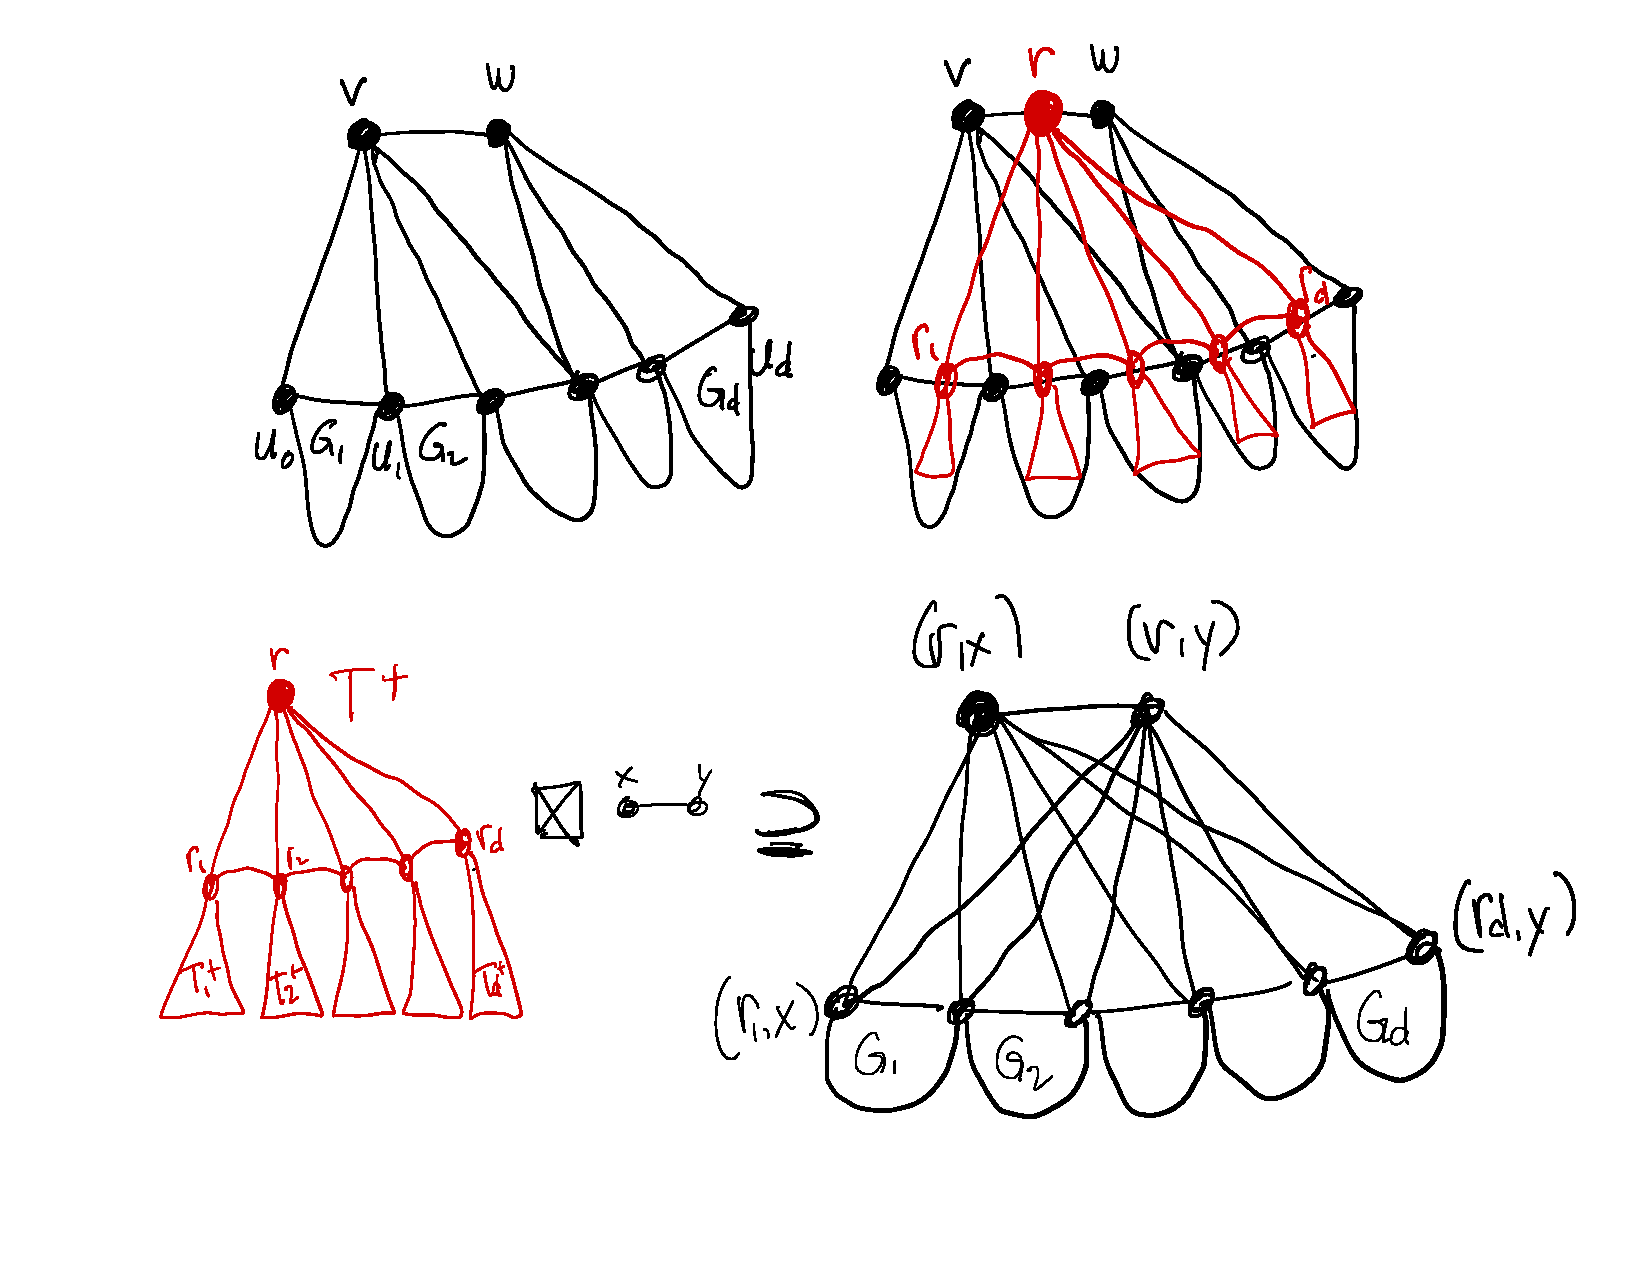
\includegraphics[width=.95\textwidth]{figs/outerplanar-product}
%     \end{center}
%     \caption{The statement of \cref{product-structure-outerplanar-technical}.}
%     \label{outerplanar-product}
% \end{figure}
%
% \begin{lem}\label{product-structure-outerplanar-technical}
%     Let $P=xy$ be a length-1 path, let $G$ be an edge-maximal outerplane graph with $|G|\ge 2$, and let $vw$ be an edge of the outer face of $G$.  Then there exists an at most $n$-node rooted ordrered tree $T$ with root $r$ and an injective function $\xi:V(G)\to V(T^+\boxtimes P)$ such that
%     \begin{compactenum}[(P1)]
%         \item $\xi(v)=(r,x)$;
%         \item $\xi(v)=(r,y)$;
%         \item for each edge $st\in E(G)$, $\xi(s)\xi(t)\in E(T^+\boxtimes P)$.
%         \item for each pair $(s,t)\in \{v,w\}\times (N_G(v)\cup N_G(w)\setminus\{v,w\})$, $\xi(w)\xi(u)\in E(T^+\boxtimes P)$.
% \end{compactenum}
% \end{lem}
%
% \begin{proof}
%     The proof is by induction on $n:=|G|$. For the base case $n=2$ and $G$ consists of a single edge $vw$.  We use the tree $T$ consisting of a single node $r$ and the function $\xi$ defined by $\xi(v)=(r,x)$, $\xi(w)=(r,y)$.  By definition this satisfies (P1) and (P2).  It satisfies (P3) because $xy\in E(P)$ so (by the definition of $\boxtimes$) $\xi(v)\xi(w)=(r,x)(r,y)\in E(T^+\boxtimes P)$. Condition (P4) is vacuously true, since $N_G(v)\cup N_G(w)\setminus\{v,w\}=\emptyset$
%
%     For $n\ge 3$, let $\{u_0,\ldots,u_d\} := N_G(v)\cup N_G(w) \setminus \{v,w\}$ ordered in the order these vertices appear on the outer face of $G$ so that the path $u_0,v,w,u_d$ is on the outer face of $G$.  For each $i\in\{1,\ldots,d\}$, let $G_i^-$ be the component of $G-\{u_{i-1},u_i\}$ that does not contain $\{v,w\}$, and let $G_i=G[\{u_{i-1},u_i\}\cup V(G_i^-)]$.  For each $i\in\{1,\ldots,d\}$, the edge $u_{i-1}u_i$ is on the outer face of $G_i$.  By applying induction on $G_i$ for each $i\in\{1,\ldots,d\}$ we obtain trees $T_1,\ldots,T_d$ with roots $r_1,\ldots,r_d$, and functions $\xi_1,\ldots,\xi_d$, where each $(T_i,\xi_i)$ satisfies the conditions of the lemma with $v=u_{i-1}$ and $w=u_i$.
%
%     Our tree $T$ will consist of a root $r$ whose children are $r_1,\ldots,r_d$. We set $\xi(v):=(r,x)$ and $\xi(w):=(r,y)$ as required by (P1) and (P2).  We set $\xi(u_0)=(r_1,x)$ and, for each $i\in\{1,\ldots,d\}$, we set $\xi(u_i)=(r_i,y)$.  For each $i\in\{1,\ldots,d\}$ and each vertex $s\in V(G_i-\{u_{i-1},u_i\})$ we set $\xi(s):=\xi_i(s)$.  To see that this satisifies (P3) and (P4), consider some pair $st\in E(G)\cup (\{v,w\}\times (N_G(v)\cup N_G(w)\setminus\{v,w\}))$.
%     \begin{enumerate}
%         \item If $st=vw$ then, $\xi(s)=(r,x)$ and $\xi(t)=(r,y)$ so $\xi(s)\xi(t)\in E(T^+\boxtimes P)$ since $xy\in E(P)$.
%
%         \item If $s=v$ and $t=u_0$ then $\xi(s)=(r,x)$ and $\xi(t) = (r_1,x)$ so $\xi(s)\xi(t)\in E(T^+\boxtimes P)$ since $rr_1\in E(T^+)$.
%
%         \item If $s=w$ and $t=u_0$ then $\xi(s)=(r,y)$ and $\xi(t) = (r_1,x)$ so $\xi(s)\xi(t)\in E(T^+\boxtimes P)$ since $rr_1\in E(T^+)$ and $xy\in E(P)$.
%
%         \item If $s=v$ and $t=u_i$ for some $i\in\{1,\ldots,d\}$, then $\xi(s)=(r,x)$ and $\xi(t)=(r_i,y)$,  so $\xi(s)\xi(t)\in E(T^+\boxtimes P)$ since $rr_i\in E(T^+)$ and $xy\in E(P)$.
%
%         \item If $s=w$ and $t=u_i$ for some $i\in\{1,\ldots,d\}$, then $\xi(s)=(r,y)$ and $\xi(t)=(r_i,y)$,  so $\xi(s)\xi(t)\in E(T^+\boxtimes P)$ since $rr_i\in E(T^+)$.
%
%         \item If $s=u_{0}$ and $w=u_{1}$ then $\xi(s)=(r_1,x)$ and $\xi(t)=(r_1,y)$,  so $\xi(s)\xi(t)\in E(T^+\boxtimes P)$ since $xy\in E(P)$.
%
%         \item If $s={u-1}$ and $w=u_i$ for some $i\in\{2,\ldots,d\}$, then $\xi(s)=(r_{i-1},y)$ and $\xi(t)=(r_i,y)$,  so $\xi(s)\xi(t)\in E(T^+\boxtimes P)$ since $r_{i-1}r_i\in E(T^+)$.
%
%         \item If $s\in\{u_{i-1},u_i\}$ and $t\in V(G_i)\setminus\{u_{i-1},u_i\}$ for some $i\in\{1,\ldots,d\}$, then $t\in N_{G_i}(u_{i-1})\cup N_{G_i}(u_i)$.  Furthermore $\xi(s)\in\{x_i(u_{i-1}),\xi_i(u_i)\}$ so, by the inductive hypothesis and (P4), $\xi(s)\xi(t)\in \xi_i(s)\xi_i(t)\in E(T_i^+\boxtimes P) \subseteq E(T^+\boxtimes P)$.
%
%         \item If $s,t\in V(G_i)\setminus\{u_{i-1},u_i\}$ for some $i\in\{1,\ldots,d\}$ then $\xi(s)=\xi_i(s)$ and $\xi(t)=\xi_i(t)$ so, by the inductive hypothesis and (P3), $\xi(s)\xi(t)\in \xi_i(s)\xi_i(t)\in E(T_i^+\boxtimes P) \subseteq E(T^+\boxtimes P)$. \qedhere
%     \end{enumerate}
% \end{proof}

\subsection{Bounded Genus Graphs}

We now prove the upper bound in \cref{bounded-genus}. To do this, we make use of the following product structure theorem of \citet{dujmovic.joret.ea:planar}:\footnote{\citet{dujmovic.joret.ea:planar} state a version of \cref{product-structure} that describes $H$ as an apex graph of treewidth at most $4$.  By definition, this means that $H$ has an apex vertex $a$ such that $H-\{a\}$ is planar.  It is not hard to see that the removal of $a$ also reduces the treewidth of $H$ to 3, yielding the version \cref{product-structure-genus} stated here.}

\begin{thm}[\cite{dujmovic.joret.ea:planar}] \label{product-structure-genus}
    For every $n$-vertex graph $G$ of Euler genus at most $g$, there exists some at most $n$-vertex path $P$, some at most $n$-vertex graph $H$, and a vertex $a\in V(H)$ such that $H-\{a\}$ is a planar 3-tree and $G$ is isomorphic to a subgraph of $H\boxtimes K_{\max\{2g,3\}}\boxtimes P$
\end{thm}

\begin{proof}[Proof of \cref{bounded-genus}]
    Apply \cref{product-structure-genus} to $G$ to obtain the graph $H$ and path $P$.  By \cref{planar} there exists a 2-ranking $\varphi:V(H-\{a\})\to \{1,\ldots,k\}$ with $k\in O(\log n/\log^{(3)} n)$. Setting $\varphi(a):=k+1$ then gives a 2-ranking of $H$, so $\trn(H)\le k+1\in O(\log n/\log^{(3)} n)$.  The same argument used in the proof of \cref{dumb} to show that $\dtcn(K_3\boxtimes P)\le 9$ shows that $\dtcn(K_{\max\{2g,3\}}\boxtimes P)\le 3\max\{2g+3\}$.  \cref{bounded-genus} now follows from \cref{product-lemma}.
\end{proof}

\subsection{Other Graph Families with Product Structure}

As noted in the introduction, several other families of graphs are known to have product structure theorems like \cref{product-structure,product-structure-genus}.  In particular, \citet{dujmovic.joret.ea:planar} show:

\begin{thm}[\cite{dujmovic.joret.ea:planar}]\label{apex-minor-free}
    For any apex graph $A$, there exists a value $t$ such that any $n$-vertex $A$-minor free graph $G$ is isomorphic to a subgraph of $H\boxtimes P$ where $H$ is an at most $n$-vertex graph of treewidth at most $t$ and $P$ is a path.
\end{thm}

\citet{dujmovic.morin.ea:structure} show a similar result for some non-minor-closed families of graphs, the most well-known of which are the $k$-planar graphs:

\begin{thm}[\cite{dujmovic.morin.ea:structure}]\label{gk-planar}
    For any integers $g$ and $k$, there exists a value $t$ such that any $n$-vertex $(g,k)$-planar graph $G$ is isomorphic to a subgraph of $H\boxtimes P$, where $H$ is an at most $n$-vertex graph of treewidth at most $t$ and $P$ is a path.
\end{thm}

\begin{proof}[Proof of \cref{meta}]
    For any $n$-vertex member $G$ of these graph families, \cref{gk-planar,apex-minor-free} show that $G$ is a subgraph of $H\boxtimes P$ with $\tw(H)\le t$.  \Cref{product-lemma,t-trees} and the fact taht $\trn(P)\le 3$ then imply \cref{meta}.
\end{proof}





% \begin{proof}[Proof of \cref{outerplanar}]
%
%
% \end{proof}
%
%
%
%
%
%
%
% % [TODO: Question: Is there a product structure theorem for outerplanar graphs?  Maybe $G\subseteq T\boxtimes P$ where $P$]
% \begin{lem}\label{outerplanar-technical}
%     Let $c,k$ be positive integers with $0\le c < k$, Let $G$ be an edge-maximal outerplane graph with outer face $F=v_1,\ldots,v_n$ and $3\le n:=|G|\le k!/c!-2$. Then, for any distinct $\phi_1,\phi_2,\phi_3\in\{a(k-c-1)+1,\ldots,ak\}$, there exists a weak 2-ranking $\varphi:V(G)\to\{1,\ldots,k\}$ such that $\varphi(v_i)=\phi_i$ for each $i\in\{1,2,3\}$.
% \end{lem}
%
% \begin{proof}
%     The proof is by induction on $n:=|G|$. The base case $n=3$ is trivial since, for any $a\ge 3$ we can colour the vertices of $G$ with the three colours $\phi_1$, $\phi_2$, and $\phi_3$.
%
%     For $n\ge 3$, let $w_1,\ldots,w_d$ denote the neighbours of $v_2$ in cyclic order, ordered so that $w_1=v_1$ and $w_d=v_3$. Then $w_1,\ldots,w_d$ is a path in $G$.  Consider the subgraph $X$ of $G$ induced by every vertex of every inner face of $G$ that is bounded by $w_iw_{i+1}$ for some $i\in\{1,\ldots,d-1\}$.
%
%     More formally, for each $i\in\{1,\ldots,d-1\}$, let
%     $Z_i$ denote the set of vertices $v$ such that $v\neq v_2$ and $vw_iw_{i+1}$ is an inner face of $G$. Observe that $|Z_i|\le 1$ since there are at most two faces bounded by $w_iw_{i+1}$ and one of these is $v_2w_iw_{i+1}$.  Then $X=G[v_2,w_1,\ldots,w_{d}\cup\bigcup_{j=1}^{i-1} Z_i]$.  We claim that $\pw(X)\le 3$.  Indeed, consider the path decomposition $(B_x:x\in P)$ where $P:=1,\ldots,d-1$ and, for each $x\in\{1,\ldots,d-1\}$, $B_x:=\{v_2,w_i,w_{i+1}\}\cup Z_i$.  Each bag $B_x$ in this path decomposition has size 4 or less.
%
%     For convenience, define $Z_0:=Z_{d+1}:=\emptyset$.  Fix some $i\in\{1,\ldots,d\}$ and consider the graph $G-\{w_{i}\}-Z_{i-1}-Z_i$.  This graph has a component $C$ that contains $v_2$ and (possibly) other components $C_1,\ldots,C_m$.  Let $G_i:=G[w_i\cup Z_{i-1}\cup Z_i\bigcup_{j=1}^m V(C_j)]$.  We say that $G_i$ is \emph{heavy} if $|G_i|-2 > k!/(c+1)!$ and let $I\subseteq\{1,\ldots,d\}$ consist of all $i$ for which $G_i$ is heavy.  Observe that $\sum_{i=1}^{d}(|G_i|-2)\le |G|-2$.  Therefore, $|I|< c+1$ so $|I|\le c$.
%
%     Let $Q=\bigcup_{i\in I}\left(Z_i\cup\{w_{i},w_{i+1}\}\right)$ be the set of vertices that bound heavy subgraph.  Now, $|Q|\le 3|I|\le 3c$.  Therefore, each vertex $v\in Q$ can be assigned a distinct colour $\varphi(v)\in\{a(k-c-1)+1,\ldots,ak\}\setminus\{\phi_1,\phi_2,\phi_3\}$, provided that $a(c+1)-3\ge 3c$ which is satisfied for $a\ge 3$.
%
%     Since $\pw(X)\le 3$, $\pw(X-Q)$ has pathwidth 3. Therefore, by \cref{pathwidth} $X-Q$ has a 2-ranking $\varphi:V(X-Q)\to\{a(k-c-2)+1,\ldots,a(k-c-1)\}$ provided that $a \ge 10\ge 3\pw(X-Q)+1$.  We can then apply induction to complete the colouring for each graph $G_i$.
% \end{proof}
%
% % The proof of \cref{outerplanar} is obtained by combining \cref{trees} with the following product structure theorem for outerplanar graphs:
% %
% % \begin{thm}\label{product-structure-outerplanar}
% %     For every $n$-vertex outerplanar graph $G$, there exists an at most $n$-vertex tree $T$ and a path $P$ of length at most $n-1$ such that $G$ is isomorphic to a subgraph of $T\boxtimes P$.
% % \end{thm}
% %
% % \begin{proof}
% %
% % \end{proof}
%
%
% \begin{proof}[Proof of \cref{outerplanar}]
%     We apply \cref{outerplanar-technical} to obtain a weak 2-ranking of $G$ with respect to the layering $L_0,\ldots,L_m$ and then triple the number of colours to obtain a 2-ranking.
%     % This is an immediate consequence of \cref{product-structure-outerplanar,product-colouring,trees}.
% \end{proof}
%
%
%     This is the proof we've been discussing with Mehrnoosh. It uses the fact that the neighbourhood of a vertex in an outerplanar graph has bounded pathwidth.
% \end{proof}

\section{Lower Bounds}
\label{lower-bounds}

Next we prove the lower bound in \cref{t-trees}.

\begin{lem}\label{apex-graph}
    Let $h,k\ge 1$ be integers, let $U$ be a graph with $\trn(U)\ge h$ and let $G$ be a graph obtained by taking $k+1$ disjoint copies $U_0,\ldots,U_k$ of $U$ and adding an apex vertex $a$ adjacent to each $v\in\bigcup_{i=0}^k V(U_i)$.  Then, for any integer $k_0\in \{1,\ldots,k\}$ and any 2-ranking of $\varphi:V(G)\to\{k_0,\ldots,k\}$, $\varphi(a) \ge k_0+1$.
\end{lem}

\begin{proof}
    Since $\trn(U_i)\ge h$, there exists $v_i\in V(U_i)$ such that $\varphi(v_i)\ge h$, for each $i\in\{0,\ldots,k\}$.  Since $|\{0,\ldots,k\}=k+1>k-k_0+1=|\{k_0,\ldots,k\}|$ the Pigeonhole Principle implies that there exists distinct $i,j\in\{0,\ldots,k\}$ such that $\varphi(v_i)=\varphi(v_j)$.  Since $v_i a v_j$ is a path in $G$, this implies that $\varphi(a)\ge \varphi(v_i)+1\ge h+1$.
\end{proof}

For a graph $U$ with and integers $h,\ell\ge 0$, we define the $(h,\ell)$-boost $U^{(h,\ell)}$ of $U$ as follows: The vertex set of $U^{(h,\ell)}$ is the disjoint union of $L_0,\ldots,L_\ell$.  The set $L_0:=\{a_0\}$ consists of a single vertex. For each $i\in\{1,\ldots,\ell\}$ and each $a\in L_{i-1}$, $U^{(h,\ell)}$ contains $h\ell+1$ disjoint copies $U_{a,0},\ldots,U_{a,h\ell}$ of $U$ and contains the edge $av$ for each $v\in\bigcup_{j=0}^{h\ell} V(U_j)$.  This determines the set $L_i=\bigcup_{a\in L_{i-1}}\bigcup_{j=0}^{h\ell} V(U_{a,j})$.

\begin{lem}\label{boost}
    For any graph $U$, any integer $\ell\ge 0$, and any $h\ge\trn(U)$, $\trn(U^{(h,\ell)})\ge h\ell +1$.
\end{lem}

\begin{proof}
    Suppose, for the sake of contradiction, that $\trn(U^{(h,\ell)})=k<h\ell+1$ and let $\varphi:V(U^{(h,\ell)})\to\{1,\ldots,k\}$ be a 2-ranking of $U_{(h,\ell)}$.  Let $L_0,\ldots,L_{\ell}$ be the partition of $V(U^{(h,\ell)})$ used in the definition of $V(U^{(h,\ell)})$.
    % (Alternatively, $L_0,\ldots,L_{\ell}$ are the breadth-first-search layers of $U^{(h,\ell)}$ rooted at $a_0$.)
    We will show by induction on $\ell-i$ that, for each $a\in L_{i}$, $\varphi(a)\ge(\ell-i)h+1$. This gives the desired contradiction since it implies that, for the unique vertex $a_0\in L_0$, $\varphi(a_0)\ge \ell h+1 > k$.

    The base case of the induction, $\ell-i=0$, is trivial; it simply asserts that $\varphi(v)\ge 1$ for each $v\in L_\ell$.  For any $i\in\{0,\ldots,\ell-1\}$ we apply the inductive hypothesis to conclude that $\varphi(v)\in\{(\ell-i-1)h+1,\ldots,k\}$ for each $v\in L_{i+1}$.  For each $a\in L_i$, the subgraph of $U^{(h,\ell)}$ induced by $a$ and its neighbours in $L_{i+1}$ contains the graph described in \cref{apex-graph} with $k_0:=(\ell-i-1)h+1$.  The conclusion of \cref{apex-graph} therefore implies that $\varphi(a)\ge k_0+h=(\ell-i)h+1$, as required.
\end{proof}

\begin{lem}\label{boost-size}
    For any graph $U$ and any integers $h,\ell \ge 1$, $|U^{(h,\ell)}| \le (|U|(h\ell))^{\ell}\cdot (1+O((|U|h\ell)^{-1})$.
\end{lem}

\begin{proof}
    It is easy to see that, for each $i\in \{0,\ldots,\ell\}$, $|L_i|=(|U|(h\ell+1))^i$.  Therefore,
    \[ |U^{h,\ell}| = \sum_{i=0}^\ell |L_i| = \sum_{i=0}^\ell (|U|(h\ell+1))^i = (|U|(h\ell))^{\ell}\cdot (1+O((|U|h\ell)^{-1}) \enspace . \qedhere
    \]
\end{proof}


\begin{lem}\label{boost-treewidth}
    For any graph $U$ and any integers $h,\ell\ge$, $\tw(U^{(h,\ell)})\le \tw(U)+1$.
\end{lem}

\begin{proof}
  Create a width-$(\tw(U)+1)$ tree-decomposition $(B_x:x\in V(T))$ of $U^{(h,\ell)}$ as follows: Start with $T$ having a single node $z_0$ with $B_{z_0}=L_0$.  For each $i\in\{1,\ldots,\ell\}$, and each $a\in L_{i-1}$, find some bag $B_z$ in the current decomposition that contains $a$, take $h+1$ disjoint copies $(A_x:x\in V(T_0)),\ldots,(A_x:x\in V(T_h))$ of some width-$t$ tree decomposition $\mathcal{T}$ of $U$.  For each $i\in\{0,\ldots,h\}$, add an edge from $z$ to any node of the tree in $T_i$ and add $a$ to every bag in $T_i$.  It is straightforward to verify that this does, indeed, give a width-$\tw(U)+1$ tree-decomposition of $U^{(h,\ell)}$.
\end{proof}


\begin{thm}\label{treewidth-lower-bound}
    For each integer $t\ge 0$, there exists $\alpha,\beta>0$
    such that, for each integer $\ell\ge 2^{2^{2^{\ddots}}}$, there exists a graph $G$, with $|G|\le (\log^{(t-1)}\ell)^{\alpha\ell}$, $\tw(G)\le t$, and $\trn(G)\ge (\beta\ell\log\ell)/\log^{(t)}(\ell\log\ell)$.
\end{thm}

\begin{proof}
    The case $t=0$ is trivial; For every $n\ge 1$, taking $G$ to be an $\ell^\ell$-vertex graph with no edges gives a graph with $\tw(G)=0$ and
    \[
        \trn(G)=1=\frac{\ell\log \ell}{\ell\log\ell} = \frac{(\ell\log \ell)}{\log^{(0)}(\ell\log\ell)} \enspace .
    \]
    This establishes the result for $t=0$ with $\alpha=\beta=1$.

    The remainder of the proof is by induction on $t$.  The base case $t=1$ has already been established by \citet{karpas.neiman.ea:on} who show that the complete $(\ell+1)$-ary tree $T$ of height $\ell-1$ has $\trn(T)\ge \ell$.  The tree $T$ has size $\sum_{i=0}^{\ell-1} (\ell+1)^i \le \ell^\ell$.
    Observe that
    \[
        \trn(T) \ge \ell = \frac{\ell\log\ell}{\log\ell} \ge \frac{\ell\log\ell}{\log(\ell\log\ell)} = \frac{\ell \log \ell}{\log^{(1)}(\ell\log\ell)}
    \]
    This establishes the result for $t=1$ with the constant $\alpha=\beta=1$.

    For $t>1$ we can apply the inductive hypothesis to obtain a graph $U$, with $\tw(U)\le t-1$, $|U|=(\log^{(t-2)}m)^{\alpha'm}$ and $\trn(U)\ge \beta' m\log m/\log^{(t-1)}(m\log m)=:h$.
    We do this with the value $m:=\log^{(2)}(\ell^\ell)/\log^{(t+1)}(\ell^\ell)=\log (\ell\log\ell)/(\log^{(t)}(\ell\log\ell))$.  Now we take the graph $G:=U^{(h,\ell)}$.  By \cref{boost-treewidth}, $\tw(U^{(h,\ell)})\le \tw(U)+1\le t$.  By \cref{boost},
    \begin{align*}
       \trn(G) & \ge \ell h+1 > \ell h\\
               & = \frac{\ell \beta' m\log m}{\log^{(t-1)}(m\log m)} \\
               & = \left(\beta'\ell m\right)\left(\frac{\log m}{\log^{(t-1)}(m\log m)}\right) \\
               & = \left(\frac{\beta'\ell \log(\ell\log\ell)}{\log^{(t)}(\ell\log\ell)}\right)\left(\frac{\log m}{\log^{(t-1)}(m\log m)}\right) \\
               & \ge \left(\frac{\beta'\ell \log\ell}{\log^{(t)}(\ell\log\ell)}\right) \left(\frac{\log m}{\log^{(t-1)}(m\log m)}\right) \\
               & \ge \frac{(\beta'/2)\ell \log\ell}{\log^{(t)}(\ell\log\ell)}
   \end{align*}
   where the final inequality holds for all $t\ge 2$ and $m\ge 1$ (which holds for all $\ell\ge 2$).

   By \cref{boost-size}, the size of $G$ is given by
   \begin{align*}
        |G| & \le \gamma\cdot \left((\log^{(t-2)}m)^{\alpha' m}\ell h\right)^\ell \\
        & = \gamma ((\log^{(t-2)}m)^{\alpha'\ell m}) (\ell^\ell) (h^\ell) \\
        & = \gamma \left(\log^{(t-2)}\left(\frac{\log(\ell\log\ell)}{\log^{(t)}(\ell\log\ell)}\right)\right)
        ^{\frac{\alpha'\ell\log(\ell\log\ell)}{\log^{(t)}(\ell\log\ell)}} \cdot (\ell^\ell) (h^\ell) \\
        & \le \gamma \left(\log^{(t-2)}(\log(\ell\log\ell))\right)
        ^{\frac{\alpha'\ell\log(\ell\log\ell)}{\log^{(t)}(\ell\log\ell)}} \cdot (\ell^\ell) (h^\ell) \\
        & = \gamma \left(\log^{(t-1)}(\ell\log\ell)\right)
        ^{\frac{\alpha'\ell\log(\ell\log\ell)}{\log^{(t)}(\ell\log\ell)}} \cdot (\ell^\ell) (h^\ell) \\
        & = \gamma (\ell\log\ell)^{\alpha'\ell} (\ell^\ell) (h^\ell) \\
        & = \ell^{(\alpha'+1)\ell + \frac{\ell\log h + \ell\log\log\ell \log\gamma}{\log\ell}} \\
        & = \ell^{(\alpha'+4)\ell}
   \end{align*}
   for all sufficiently large $\ell$.
\end{proof}

Rewriting \cref{treewidth-lower-bound} in terms of $n:=|G|$, we obtain a more-readily digestible corollary:

\begin{cor}\label{treewidth-lower-bound-n}
    For every integer $t\ge 0$, there exists a constant $\alpha>0$ such that, for infinitely many $n\in\N$,   there exists an $n$-vertex graph $G$ with $tw(G)\le t$ and  $\trn(G)\ge \alpha\log n/\log^{(t+1)} n$.
\end{cor}

\begin{proof}[Proof of \cref{planar} (lower bound)]
    By \cref{treewidth-lower-bound-n}, there exists $n$-vertex 2-trees $G$ with $\trn(G)\in O(\log n/\log^{(3)} n)$.  Since every 2-tree is planar, such $G$ establish the lower bound in \cref{planar}.
\end{proof}

\begin{proof}[Proof of \cref{simple-t-trees} (lower bound)]
    By \cref{treewidth-lower-bound-n}, there exists $n$-vertex graphs $G$ with $\tw(G)=t-1$ and $\trn(G)\in\Omega(\log n/\log^{(t)} n)$.  By \cref{simple-treewidth-vs-treewidth} $\stw(G)\le t$.
\end{proof}

\section{Discussion}
\label{conclusion}

We have given asymptotically optimal bounds on the number of colours required by $2$-rankings of $n$-vertex $t$-trees, planar 3-trees, outerplanar graphs, and planar graphs.  Prior to this work, the best known bounds were $\Omega(n/\log n)$ (trees) and $O(\log n)$.

Our upper bounds are constructive and lead to $O(n)$ time algorithms for finding $2$-rankings of $t$-trees, planar 3-trees, and outerplanar graphs.  For planar graphs, we require an algorithic version of \cref{product-structure}. Currently, the fastest such algorithm runs in $O(n\log n)$ time \cite{morin:fast}.

Two directions for future work stand out:
\begin{inparaenum}[(i)]
    \item This paper settles many questions related to $2$-ranking.  How much (if any of this) can be extended to $\ell$-ranking for $\ell>2$.
    \item For constant $d$, the lower and upper bounds for 2-ranking $d$-degenerate graphs are $\Omega(n^{1/3})$ and $O(\sqrt{n})$, respectively.  Closing this gap is an intriguing open problem.
\end{inparaenum}

\section{Other Ideas}

\begin{itemize}
\item Approximation algorithm for trees, $t$-trees, and planar graphs.  Constant factor approximation algorithms for trees look easy just using a greedy strategy (any tree that needs $2k$ colours contains a complete $k$-ary tree of height $k$).  Does this extend to $t$-trees.
\end{itemize}


\section*{Acknowledgement}

The authors are grateful to David R. Wood who, after reading an early draft of this paper, pointed us to the notion of simple treewidth, which greatly simplifies the exposition.


\bibliographystyle{plainnat}
\bibliography{us}

\end{document}
